\documentclass[t]{beamer}

%\usetheme{TuringLight}
\usetheme{TuringDark}

\usepackage{tabularx}
\newcolumntype{R}{>{\raggedleft\fontsize{\blockbodysize}{\bodylineheightmultiplier\blockbodysize}\selectfont\arraybackslash}X}
\newcolumntype{L}{>{\fontsize{\blockbodysize}{\bodylineheightmultiplier\blockbodysize}\selectfont\arraybackslash}l}

\usepackage{xcolor}
\definecolor{fadedcolor}{rgb}{0.7, 0.7, 0.7}
\newcommand{\faded}[1]{\textcolor{fadedcolor}{#1}}

% Presentation data
\title{Benchmarking AI applications on GPUs}
\author{Tomas Lazauskas, David Llewellyn-Jones}
\def\cornerimagefilename{baskerville.jpg}

\newcommand\includegraphicsfullpage[1]
{
\begin{tikzpicture}[remember picture,overlay]
  \node[at=(current page.center)] {
    \includegraphics[width=1.0\paperwidth,keepaspectratio]{#1}
  };
\end{tikzpicture}
}


% Uncomment any of these lines below to set custom size for each of the font sizes.
% The default value is shown in the comment.
%\setlength{\titlefontsize}{6.875\basefontsize}
%\setlength{\subtitlefontsize}{4.375\basefontsize}
%\setlength{\frametitlesize}{2.625\basefontsize}
%\setlength{\framesubtitlesize}{1.625\basefontsize}
%\setlength{\bodytextsize}{2\basefontsize}
%\setlength{\blocktitlesize}{\bodytextsize}
%\setlength{\blockbodysize}{\bodytextsize}

\setbeamerfont*{itemize/enumerate body}{size=\fontsize{\blockbodysize}{\bodylineheightmultiplier\blockbodysize}}

% Start document
\begin{document}

% Title slide (details filled from presentation data fields above)
\begin{frame}
	\titlepage
\end{frame}

% Section divider slide
\section{Overview}

\begin{frame}{HPC Benchmarking}

\begin{enumerate}
  \item There are existing benchmarks such as MLPerf
  \begin{itemize}
    \item Mattson {\it et al.}, ``MLPerf Training Benchmark,'' {\it Proceedings of the 3rd MLSys Conference}, Austin, TX, USA, 2020
  \end{itemize}
  \item We wanted to explore real-world training performance
  \item Focus on GPT-2 (minGPT)
  \item Use PyTorch Lightning for multi-GPU strategies
  \begin{itemize}
      \item \url{https://github.com/Lightning-Universe/lightning-GPT}
  \end{itemize}
\end{enumerate}

\end{frame}

\begin{frame}{HPC Systems}
\fontsize{\blockbodysize}{\bodylineheightmultiplier\blockbodysize}\selectfont

\begin{center}
\begin{tabularx}{1.0\textwidth}{L L L L R L R}
  \hline
  Service & Name & Type & Accelerator & Mem (GB) & Interface & Launched \\ \hline
  JADE 2 & J-V100-32 & GPU & Nvidia V100 & 32 & SXM2 & 06-2017 \\
  Baskerville & B-A100-40 & GPU & Nvidia A100 & 40 & SXM4 & 06-2020 \\
  Baskerville & B-A100-80 & GPU & Nvidia A100 & 80 & SXM4 & 06-2020 \\
  Stanage & S-H100-80 & GPU & Nvidia H100 & 80 & PCIe 4.0 & 03-2023 \\
  COSMA8 & C-MI100-32 & GPU & AMD MI100 & 32 & PCIe 4.0 & 11-2020 \\
  COSMA8 & C-MI210-64 & GPU & AMD MI210 & 64 & PCIe 4.0 & 03-2022 \\
  Graphcore & IPU-POD 16 & IPU & IPU-M2000 & 14.4 & RoCEv2 & 03-2021 \\
  \faded{Dawn} & \faded{D-M1550-128} & \faded{GPU} & \faded{Intel Max 1550} & \faded{128} & \faded{PCIe 5.0} & \faded{03-2023} \\ \hline
\end{tabularx}
\end{center}

\end{frame}

\begin{frame}{}
\includegraphicsfullpage{jade2-baskerville.jpg}
\end{frame}

\begin{frame}{}
\includegraphicsfullpage{cosma8-graphcore.jpg}
\end{frame}

\begin{frame}{HPC Peak Performance on paper (TFLOPs)}

\begin{center}
\begin{tabularx}{1.0\textwidth}{L L R R R R}
  \hline
  Service & Name & FP16 & BFLOAT16 & FP32 & FP64 \\ \hline
  JADE 2 & J-V100-32 & 31.33 & -- & 15.7 & 7.8 \\
  Baskerville & B-A100-40 & 77.97 & 312 & 19.5 & 9.7 \\
  Baskerville & B-A100-80 & 77.97 & 312 & 19.5 & 9.7 \\
  Stanage & S-H100-80 & 204.9 & 1513 & 51 & 26 \\
  COSMA8 & C-MI100-32 & 184.6 & 92.3 & 23.1 & 11.5 \\
  COSMA8 & C-MI210-64 & 181 & 181 & 22.6 & 22.6 \\
  Graphcore & IPU-POD 16 & 3994 & - & 998 & -- \\
  \faded{Dawn} & \faded{D-M1550-128} & \faded{52.43} & \faded{832} & \faded{52.43} & \faded{52.43} \\ \hline
\end{tabularx}
\end{center}

\end{frame}

% Section divider slide
\section{Training}

\begin{frame}{GPT-2 model sizes used for training}

\begin{center}
\begin{tabularx}{1.0\textwidth}{L R R R R R}
  \hline
  Model & Hidden layers & Attention heads & Embedding dim & Parameters (M) & 16 bit Size (MB) \\ \hline
  GPT2 & 12 & 12 & 768 & 85.21 & 170.51 \\
  GPT2-M & 24 & 16 & 1024 & 302.51 & 605.16 \\
  GPT2-L & 36 & 20 & 1280 & 708.64 & 1417.45 \\
  GPT2-XL & 48 & 25 & 1600 & 1475.87 & 2951.96 \\
  GPT2-XXL & 60 & 30 & 1920 & 2656.08 & 5312.43 \\
  GPT2-XXXL & 84 & 40 & 2560 & 6609.33 & 12219.00 \\ \hline
\end{tabularx}
\end{center}

\end{frame}

\begin{frame}{}
\includegraphicsfullpage{gpt2-models.png}
\end{frame}

% Section divider slide
\section{Strategies}

\begin{frame}{Distributed Data Parallel\vphantom{p}}
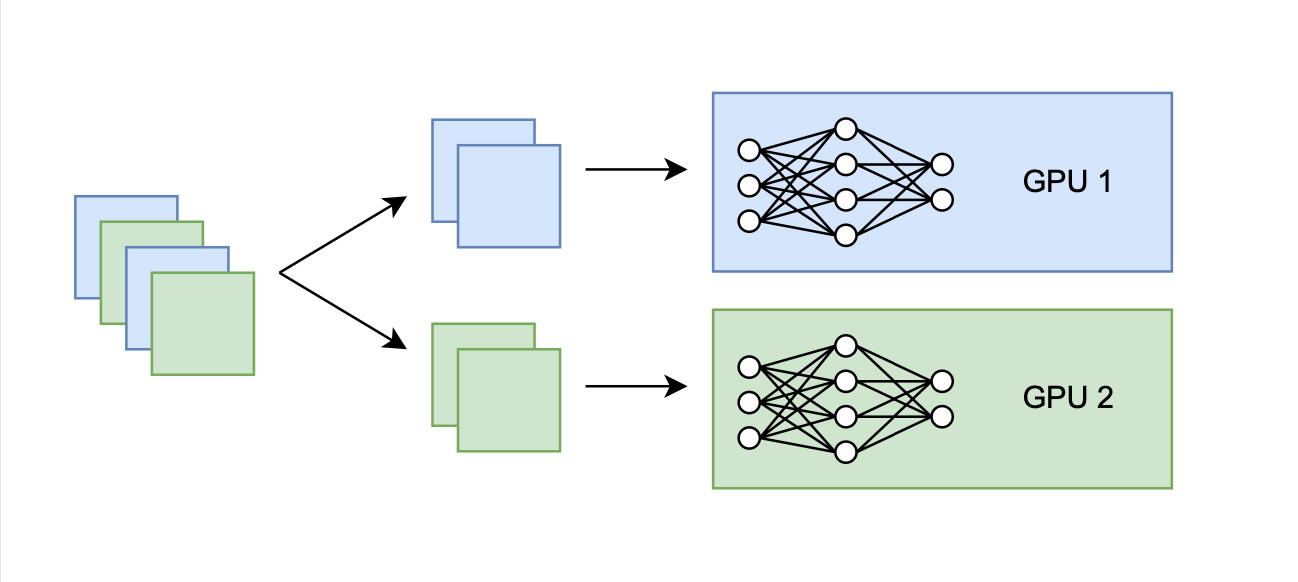
\includegraphics[width=1.0\textwidth,keepaspectratio]{1_1_DDP.png}
\end{frame}

\begin{frame}{DeepSpeed ZeRO}
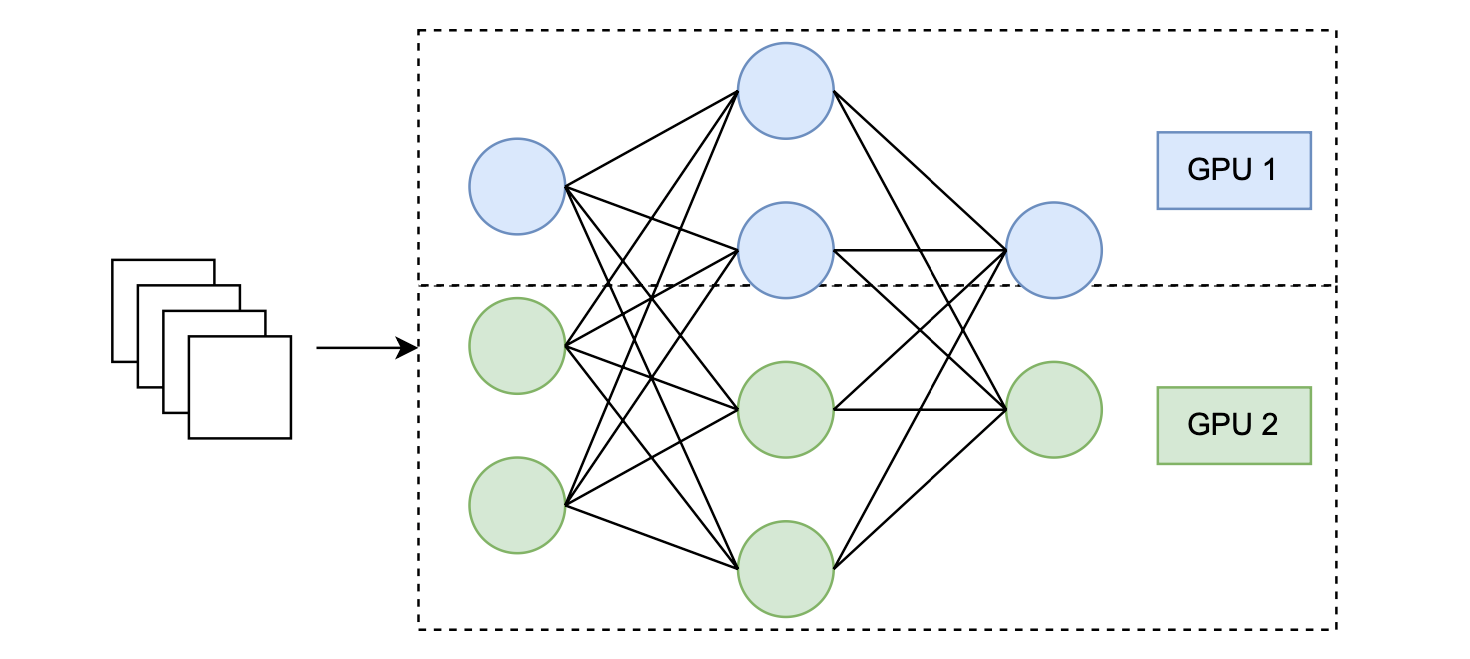
\includegraphics[width=1.0\textwidth,keepaspectratio]{1_2_horizontal.png}
\end{frame}

\begin{frame}{Fully Sharded Data Parallel}
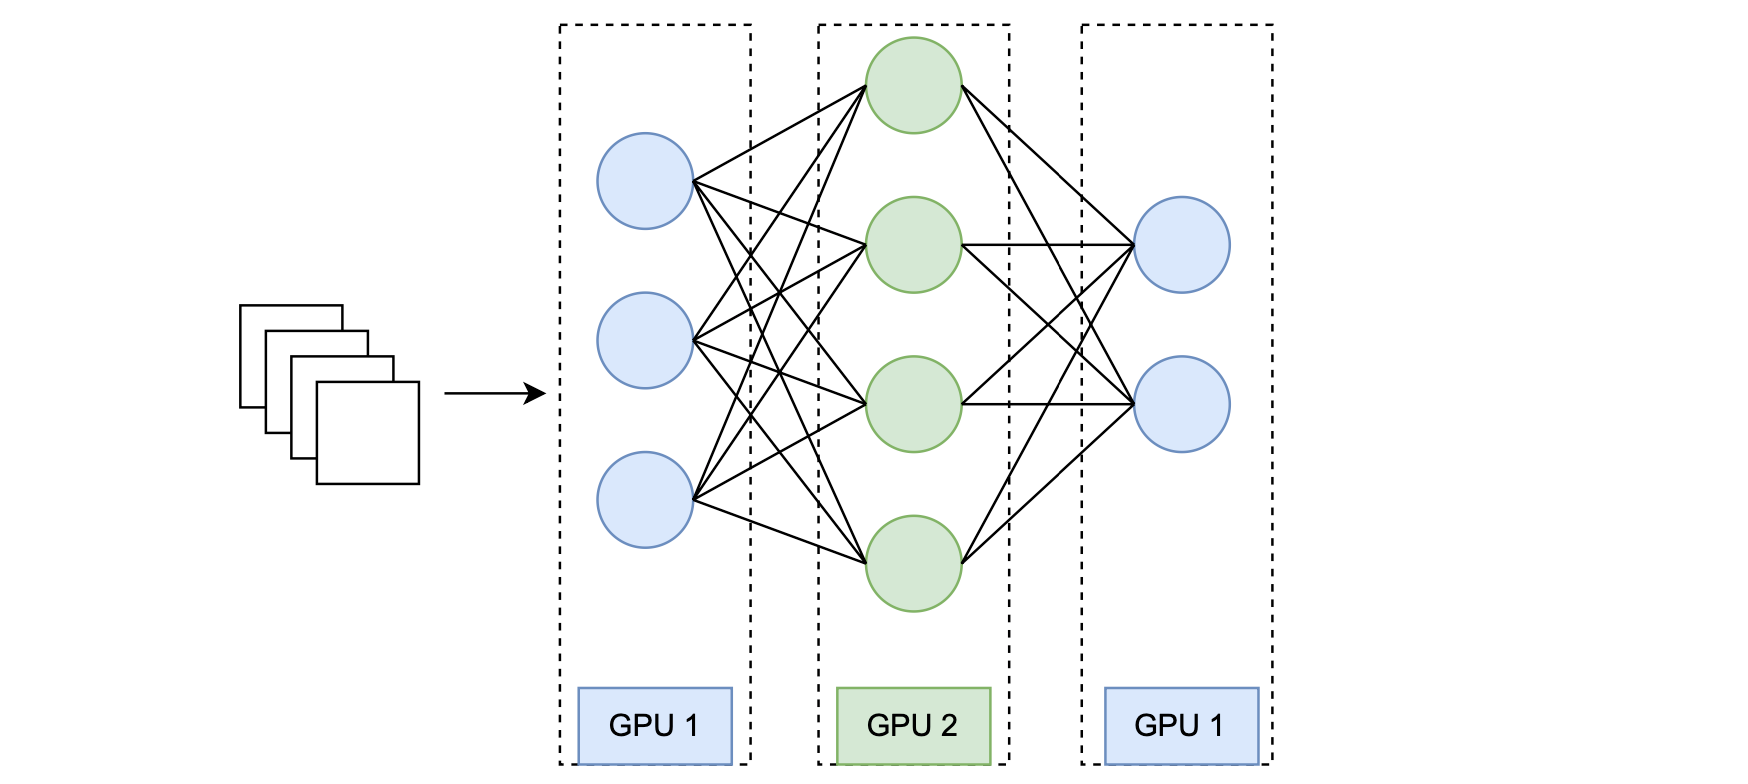
\includegraphics[width=1.0\textwidth,keepaspectratio]{1_3_vertical.png}
\end{frame}

\begin{frame}{IPU Pipelined Execution}
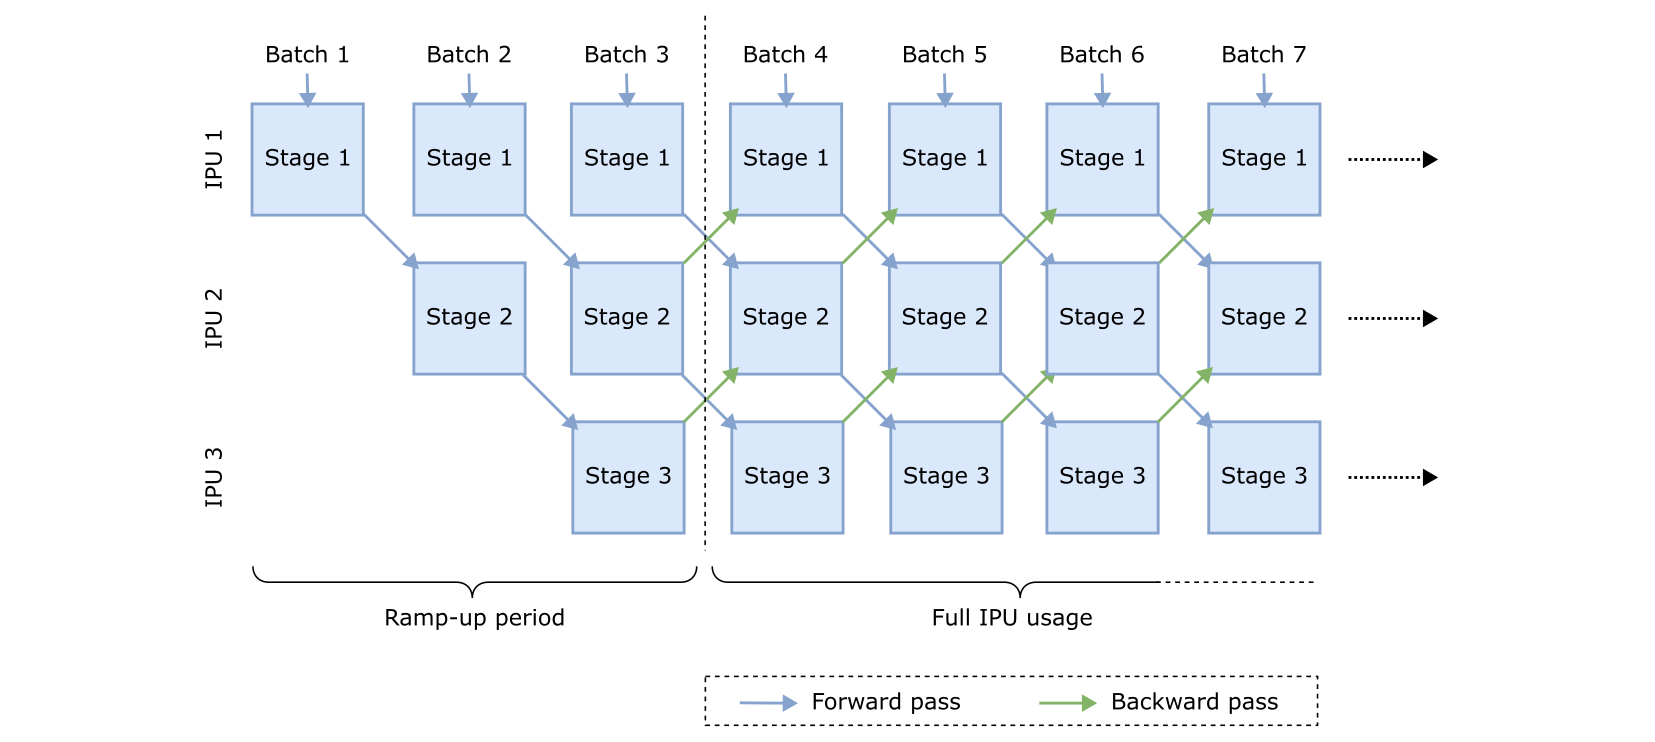
\includegraphics[width=1.0\textwidth,keepaspectratio]{6_1_1.png}
\end{frame}

\begin{frame}{IPU Sharded Execution\vphantom{p}}
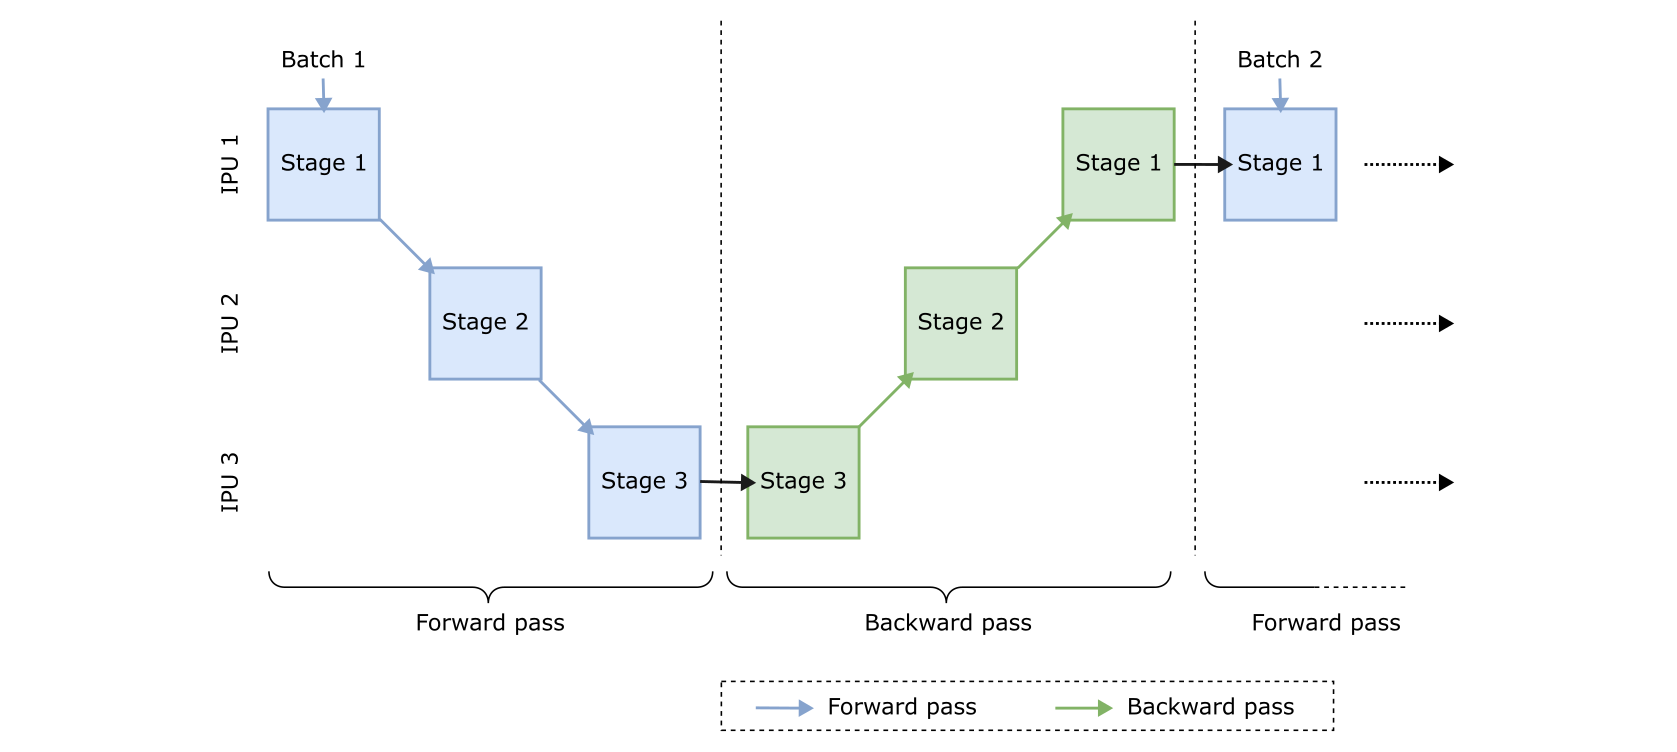
\includegraphics[width=1.0\textwidth,keepaspectratio]{6_1_2.png}
\end{frame}



% Section divider slide
\section{Single Accelerator Comparison}

\begin{frame}{Single Accelerator Comparison}
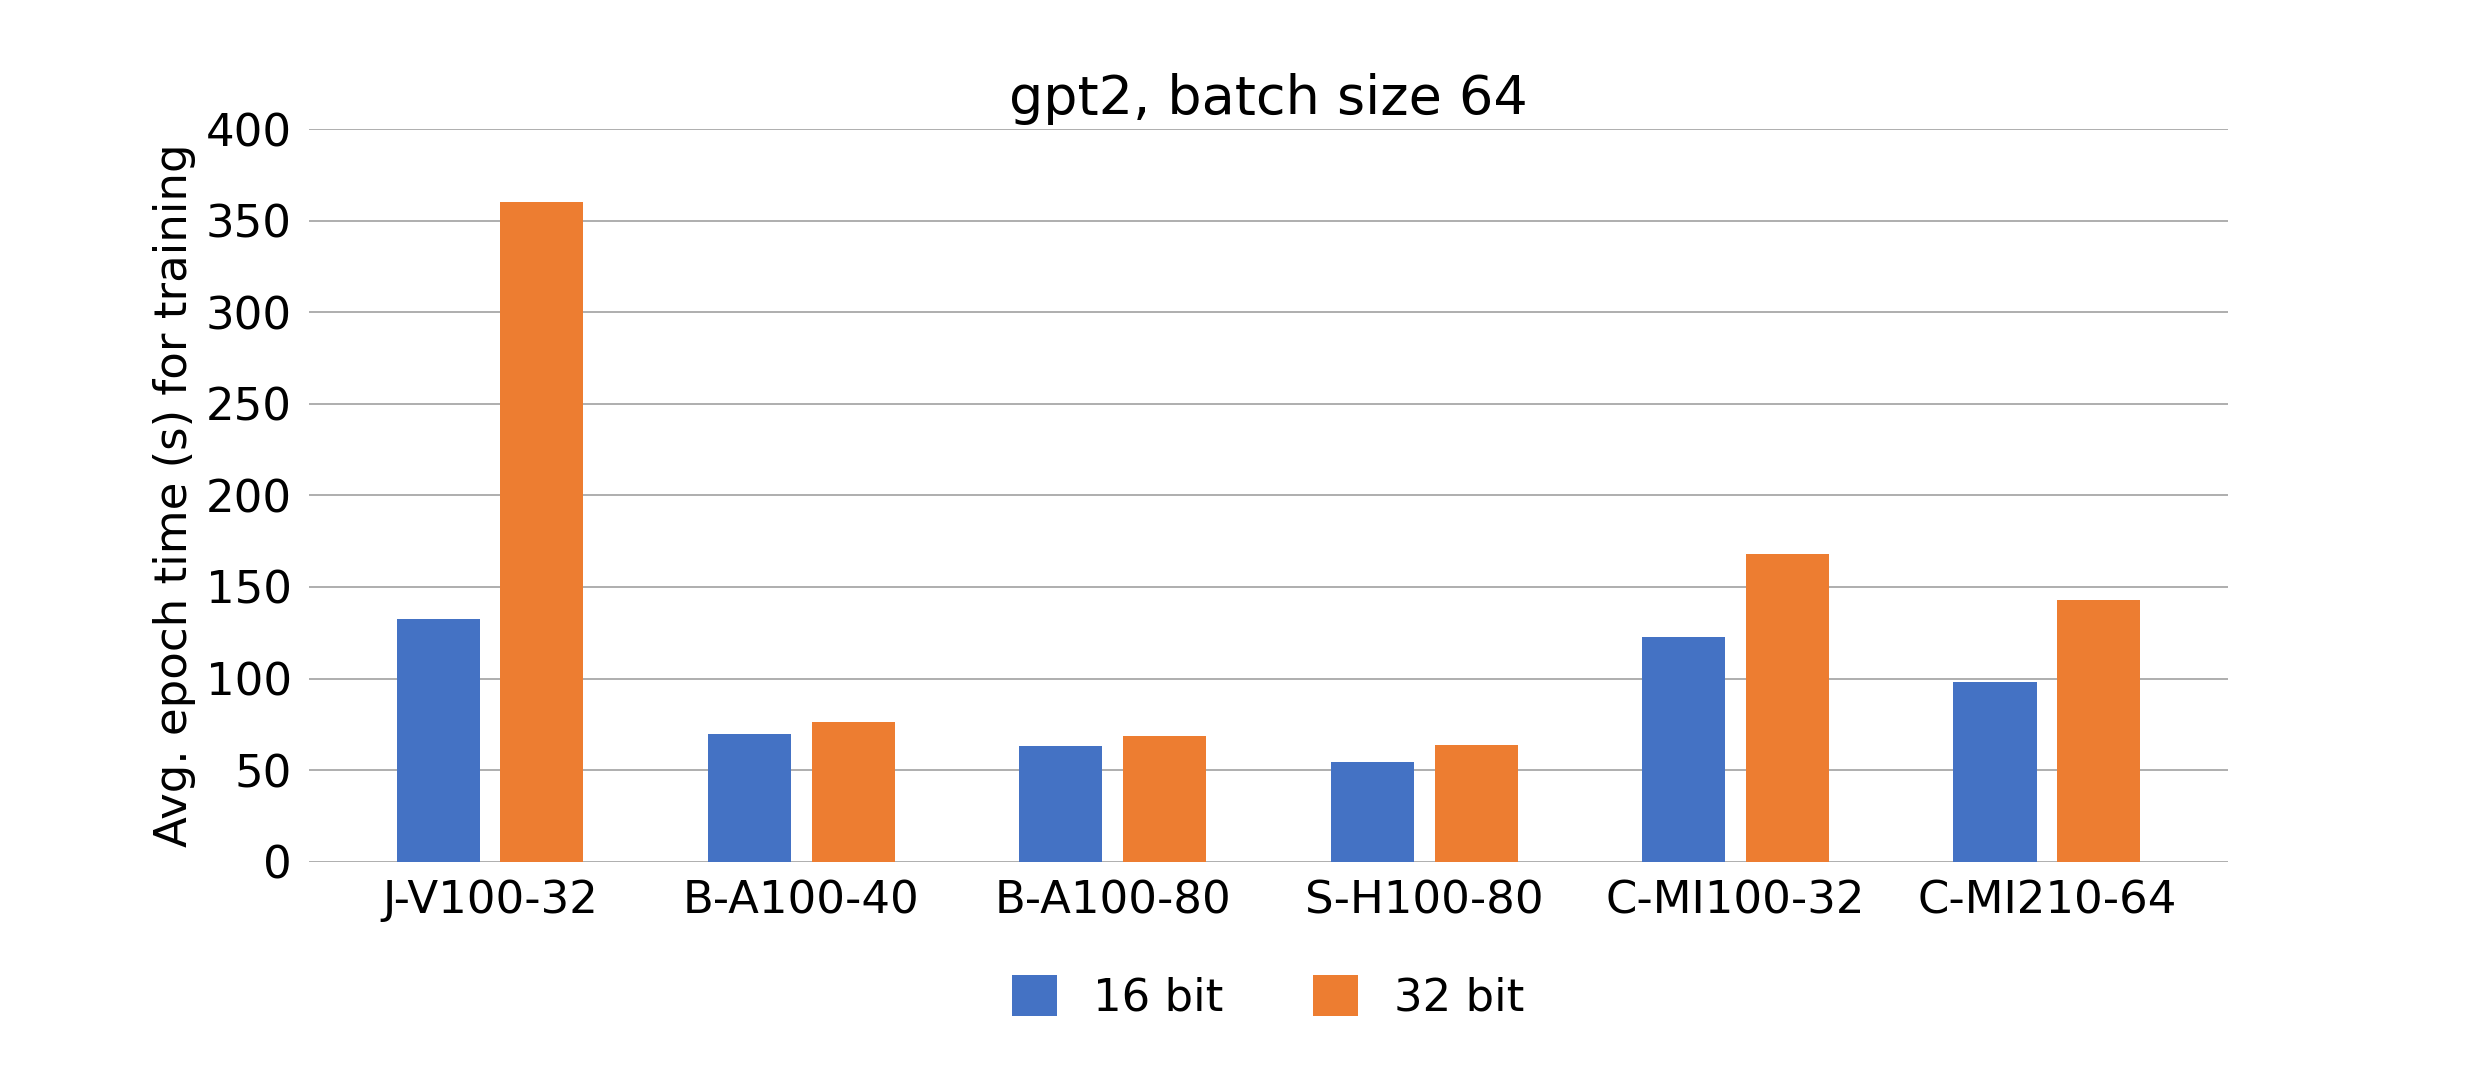
\includegraphics[width=1.0\textwidth,keepaspectratio]{2_1.png}
\end{frame}

\begin{frame}{Single Accelerator Comparison}
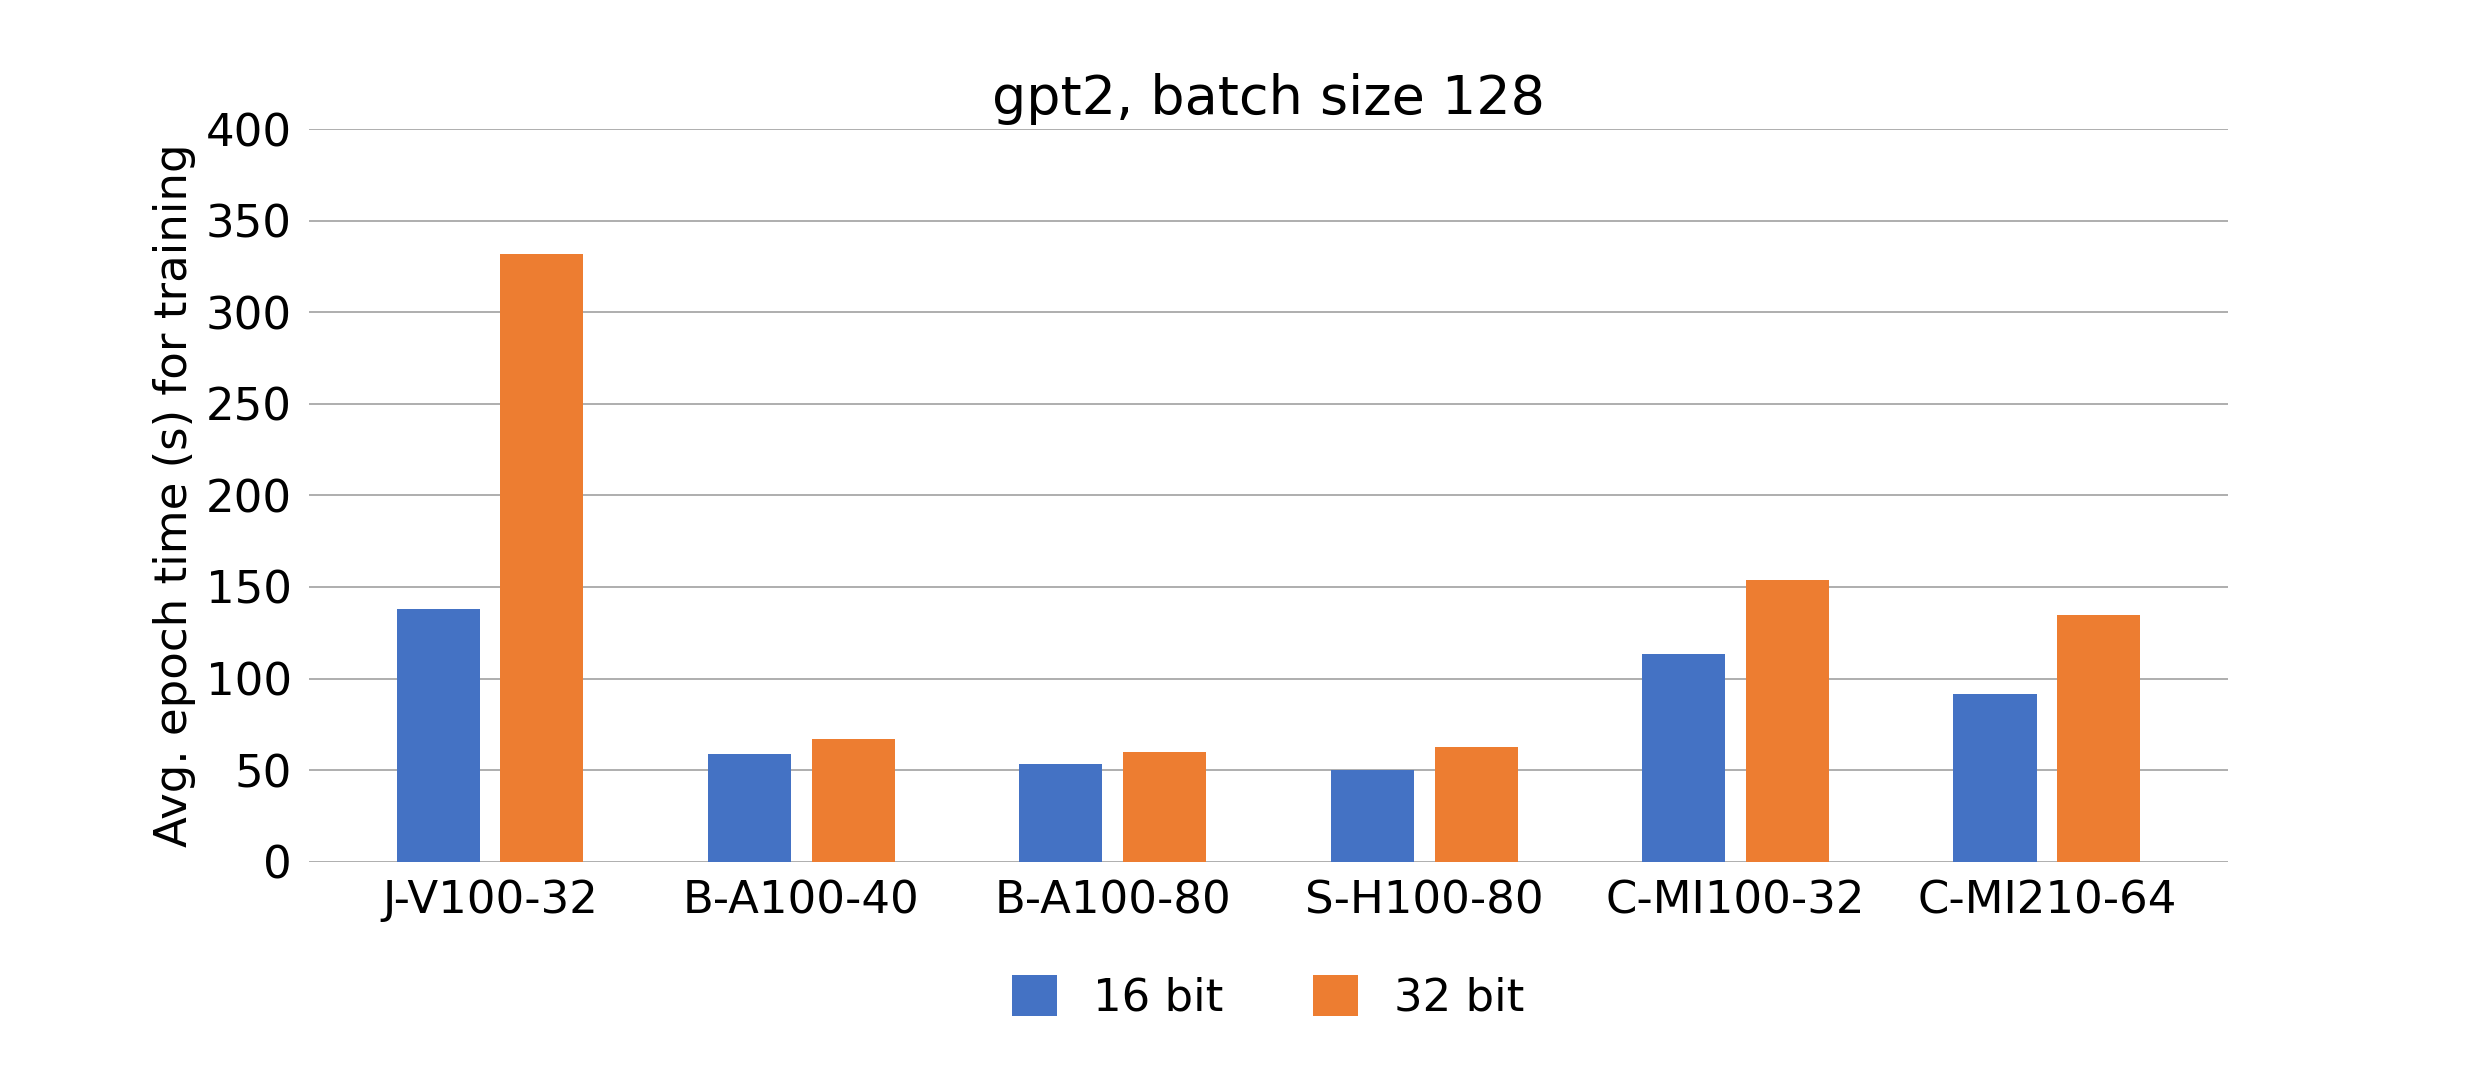
\includegraphics[width=1.0\textwidth,keepaspectratio]{2_2.png}
\end{frame}

\begin{frame}{Single Accelerator Comparison}
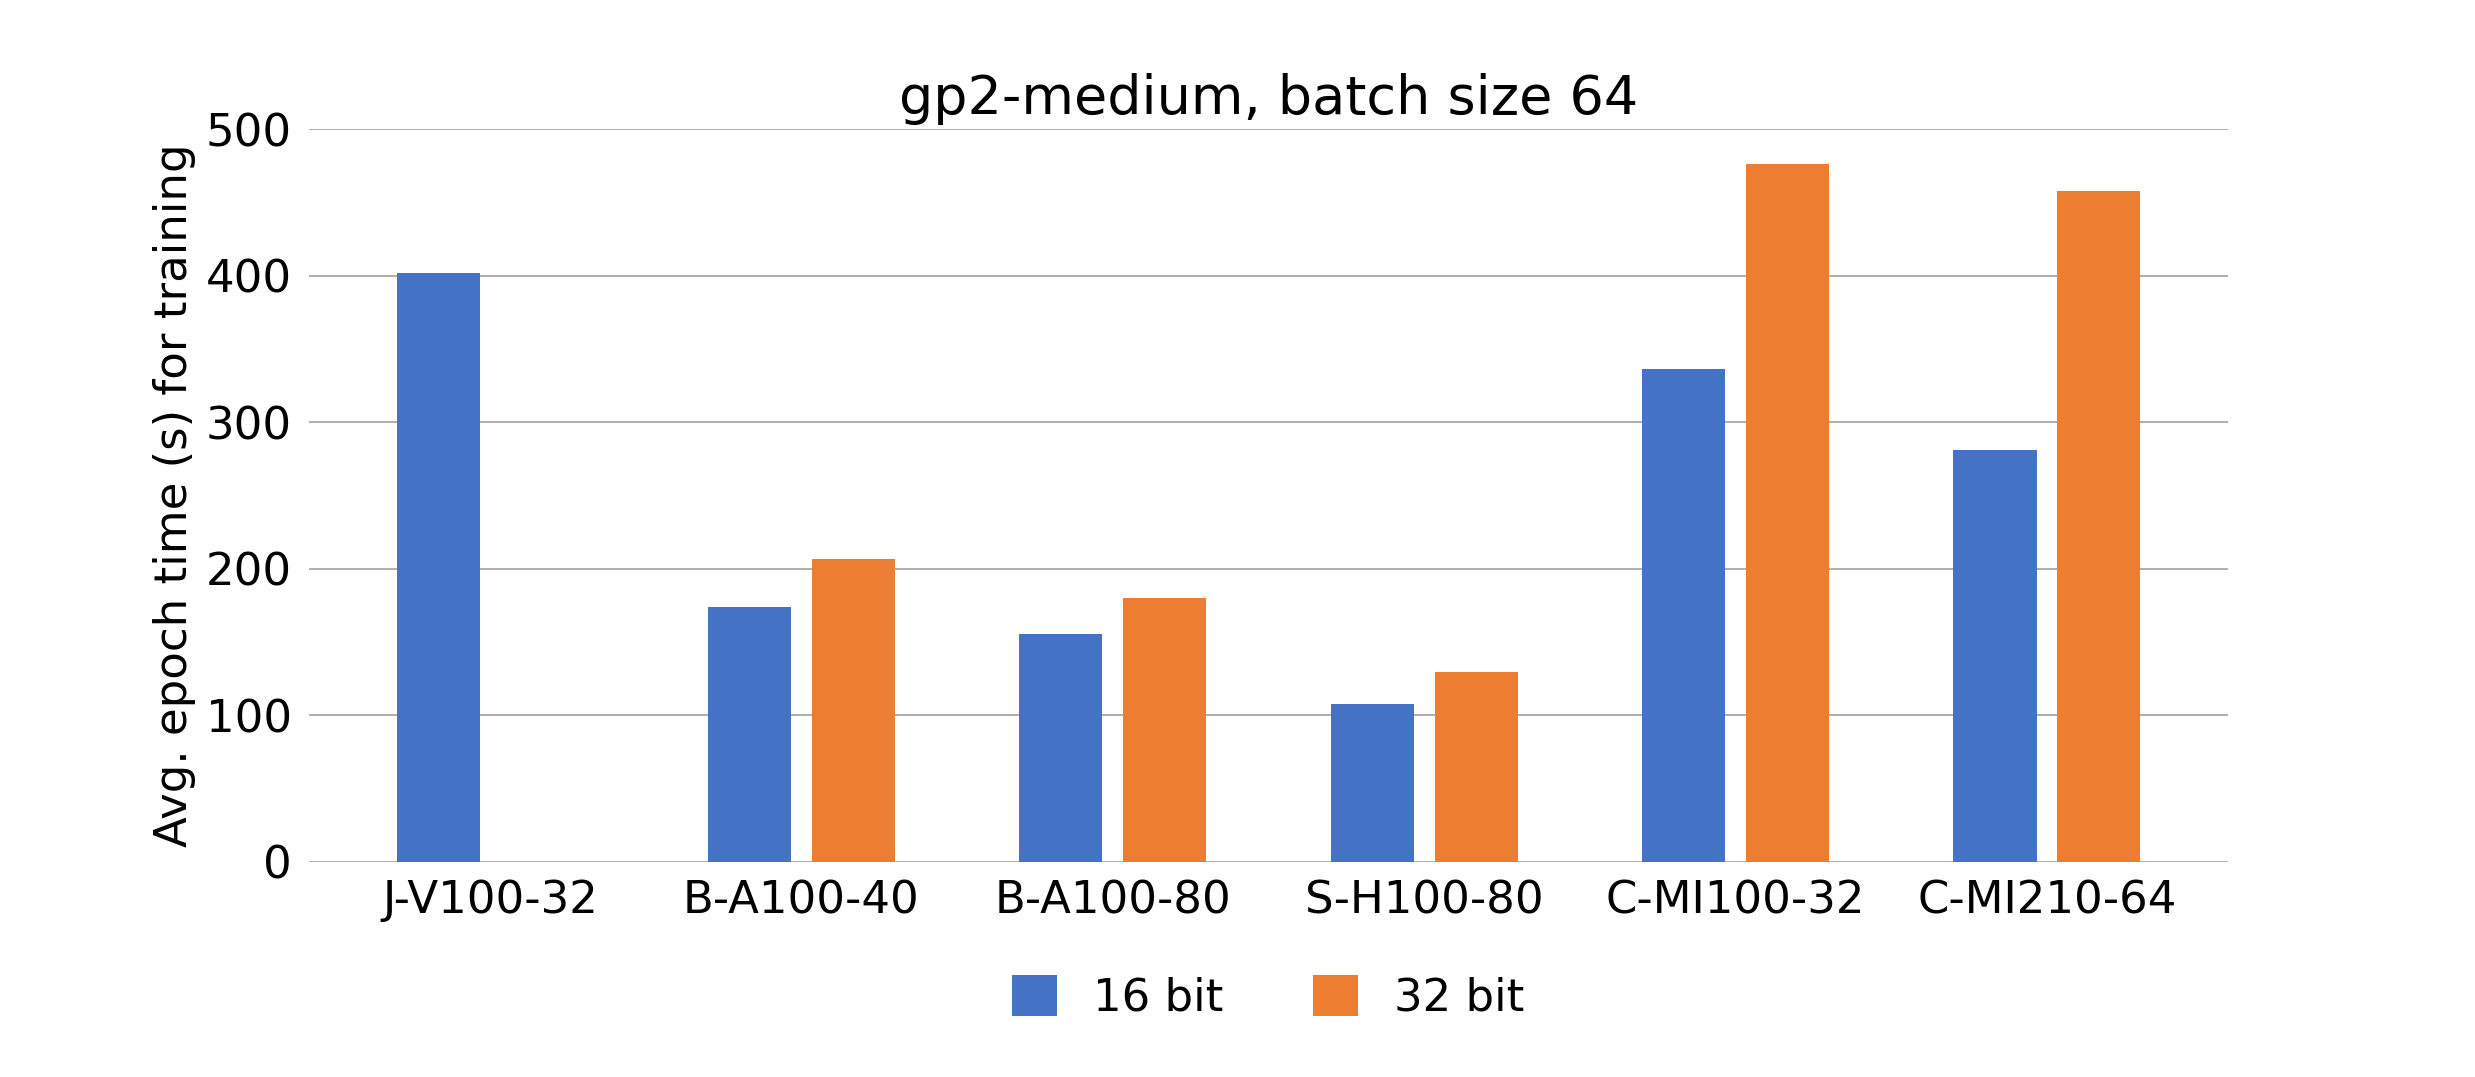
\includegraphics[width=1.0\textwidth,keepaspectratio]{2_3.png}
\end{frame}

\begin{frame}{Single Accelerator Comparison - Observations}

\begin{enumerate}
  \item S-H100-80 is the fastest GPU in terms of theoretical and actual performance.
  \item Although the S-H100-80 give the best performance, the performance gap between this and the B-A100s was not as large as we'd expected. 
  \item Performance largely depends on peak performance and precision used.
  \item Reported peak FP16 and FP32 performances don't reflect our observations.
  \item Difference between 16 bit and 32 bit precision, except for J-V100-32, is less significant when training smaller models.
  \item Increasing from GPT2 to GPT2-M results in a significant increase in training time.
  \item Doubling the batch size from 64 to 128 does not significantly improve training time.
  \item GPT2-M and a batch size of 128 wouldn't fit into 40 GB.
\end{enumerate}

\end{frame}

% Section divider slide
\section{Scaling Up and Out with DDP}

\begin{frame}{Scaling Up and Out with DDP}
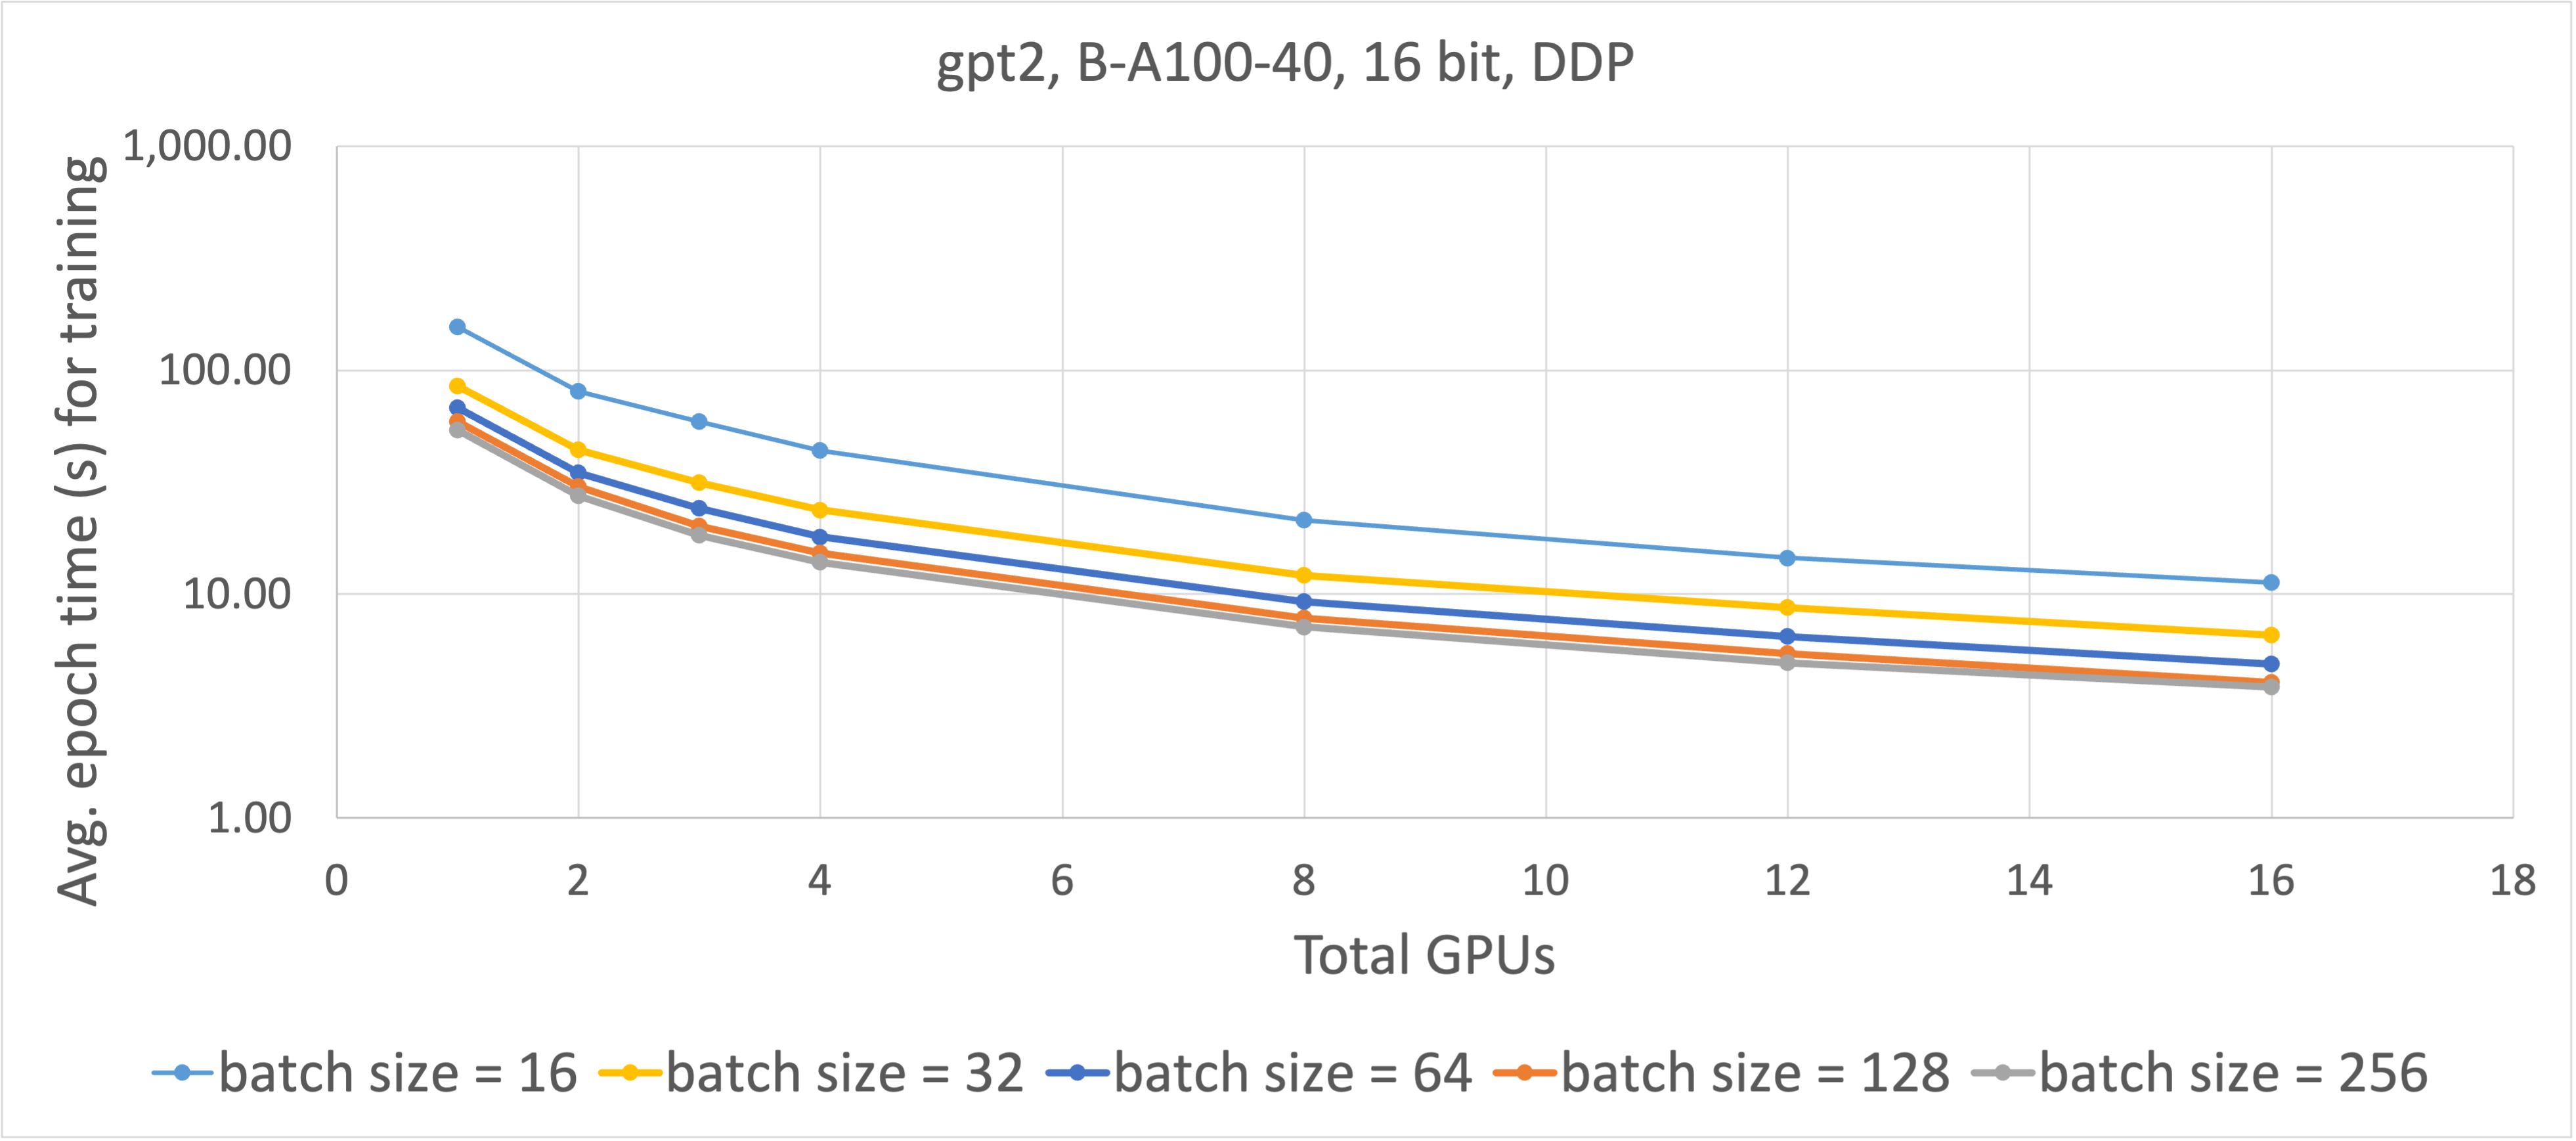
\includegraphics[width=1.0\textwidth,keepaspectratio]{3_1.png}
\end{frame}

\begin{frame}{Scaling Up and Out with DDP}
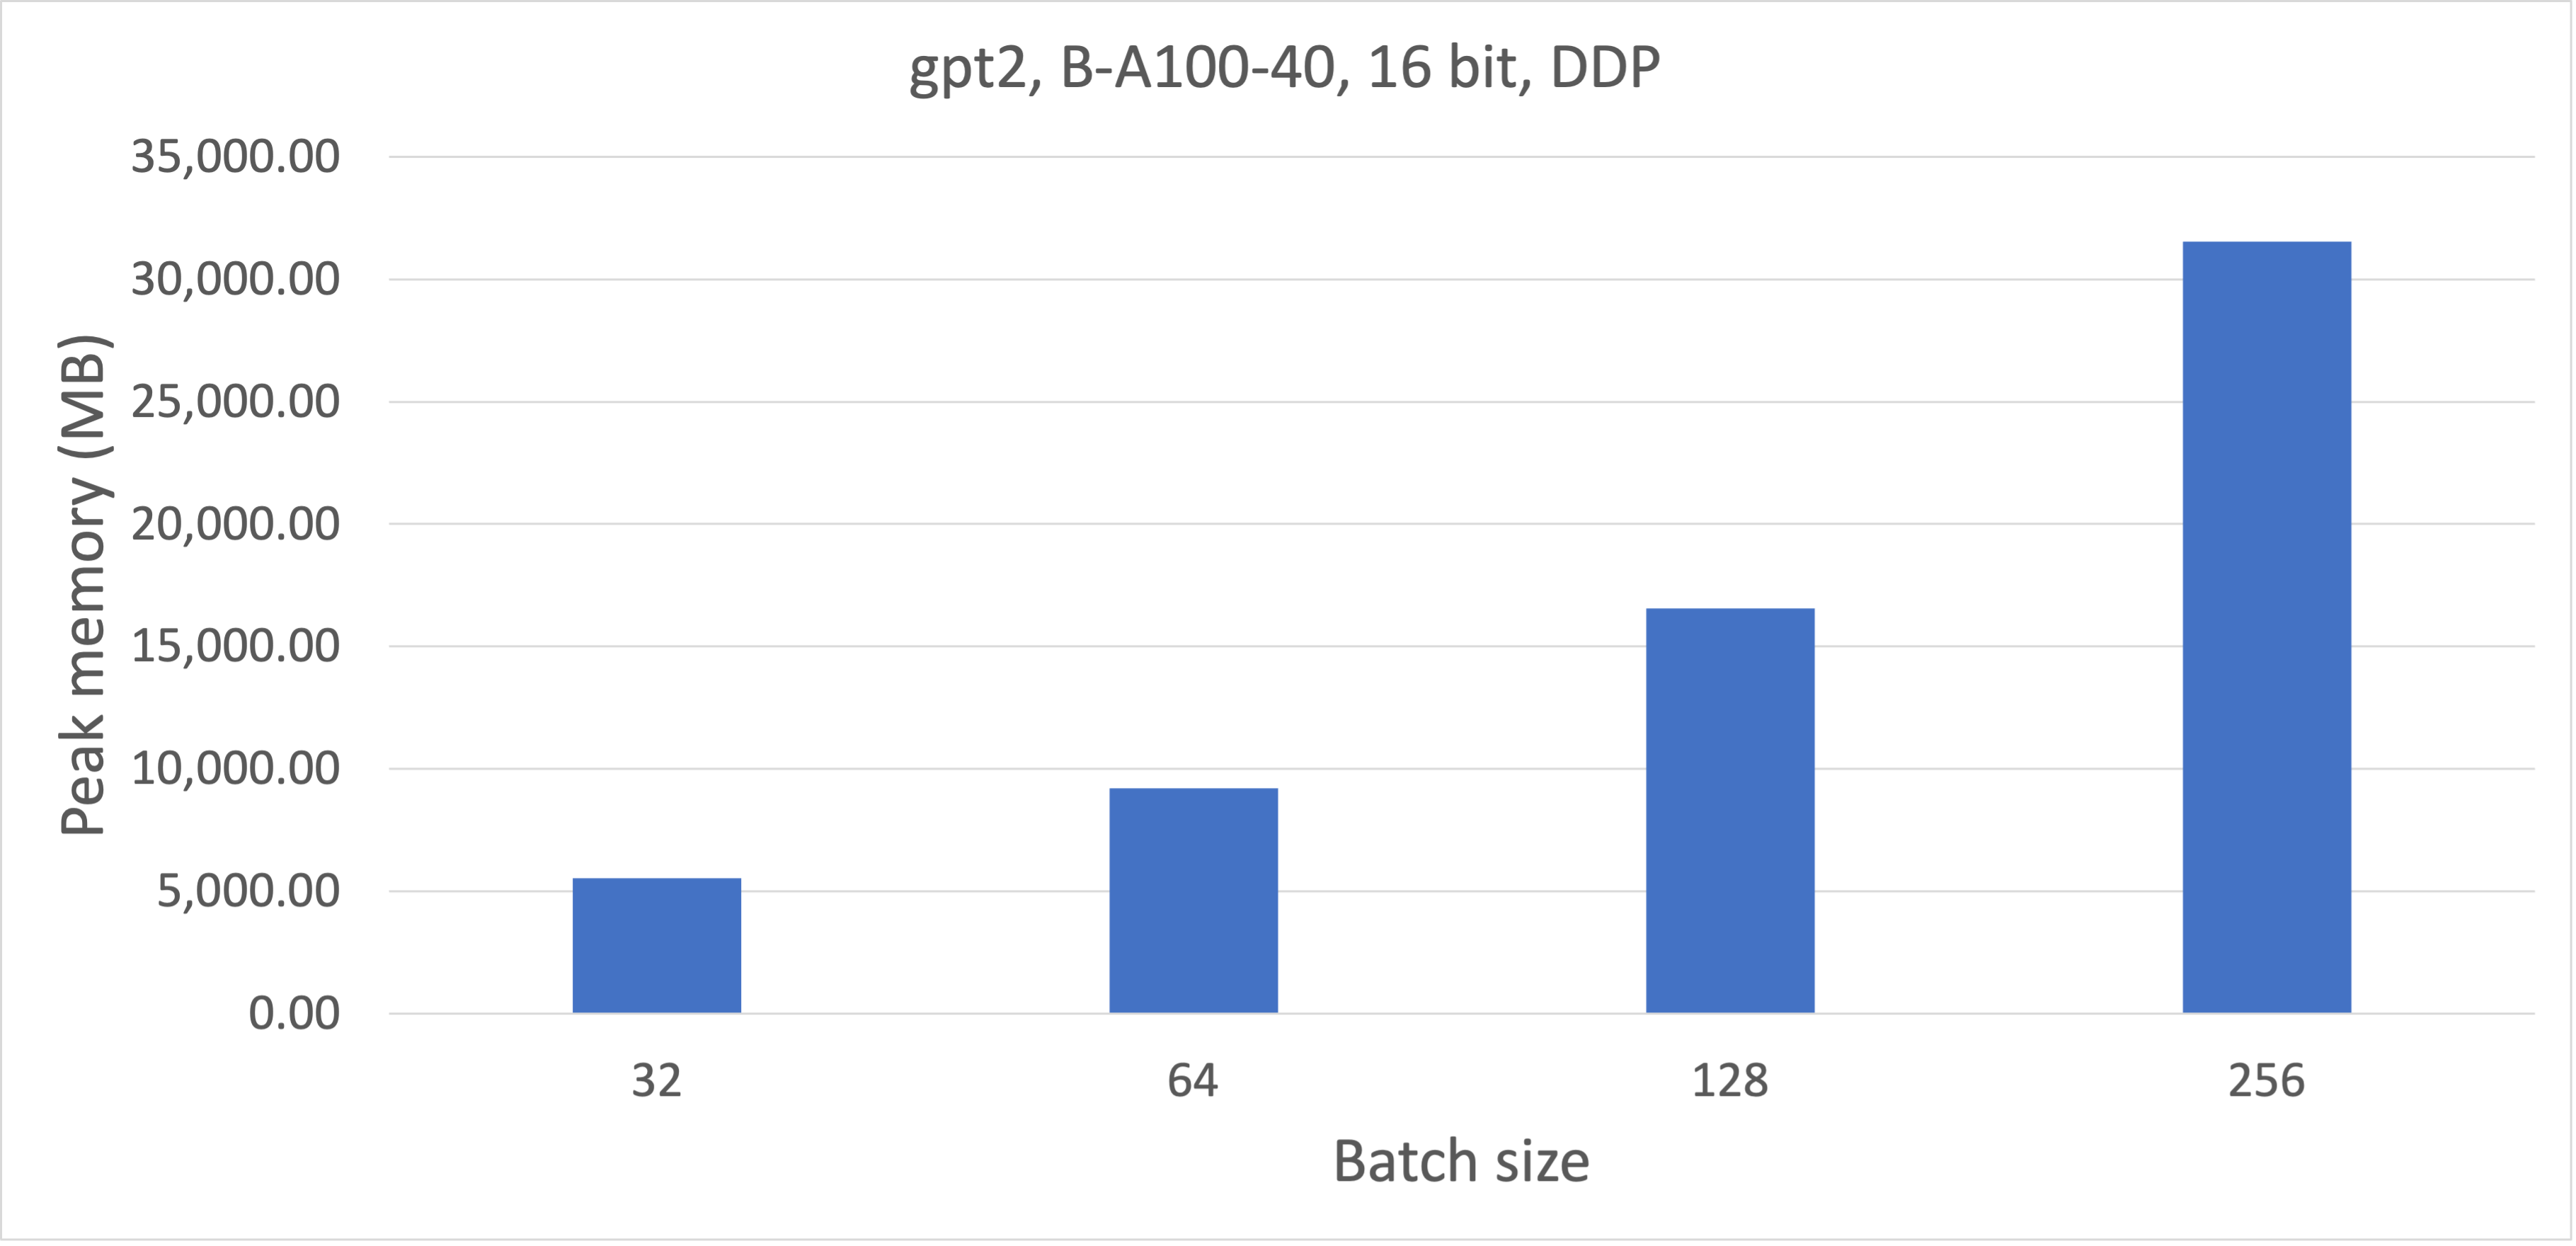
\includegraphics[width=1.0\textwidth,keepaspectratio]{3_2.png}
\end{frame}

\begin{frame}{Scaling Up and Out with DDP - Observations}

\begin{enumerate}
  \item The scaling between 1 and 16 GPUs is almost linear.
  \item Doubling batch size from 64 to 128 training time decreases by 15\%.
  \item Quadrupling from 64 to 256 training time reduces by 22\%.
  \item Halving batch size from 64 to 32 training time increases by 31\%.
  \item Quartering from 64 to 16 training time increases by 137\%.
  \item For fixed model size the limiting performance factor is the batch size.
  \item Batch size is limited by GPU memory.
  \item Doubling batch size increases the peak memory usage by a factor of 1.5.
  \item Peak memory usage did not significantly change between 1 to 16 GPUs.
\end{enumerate}

\end{frame}

% Section divider slide
\section{Larger Datasets}

\begin{frame}{Larger Datasets}
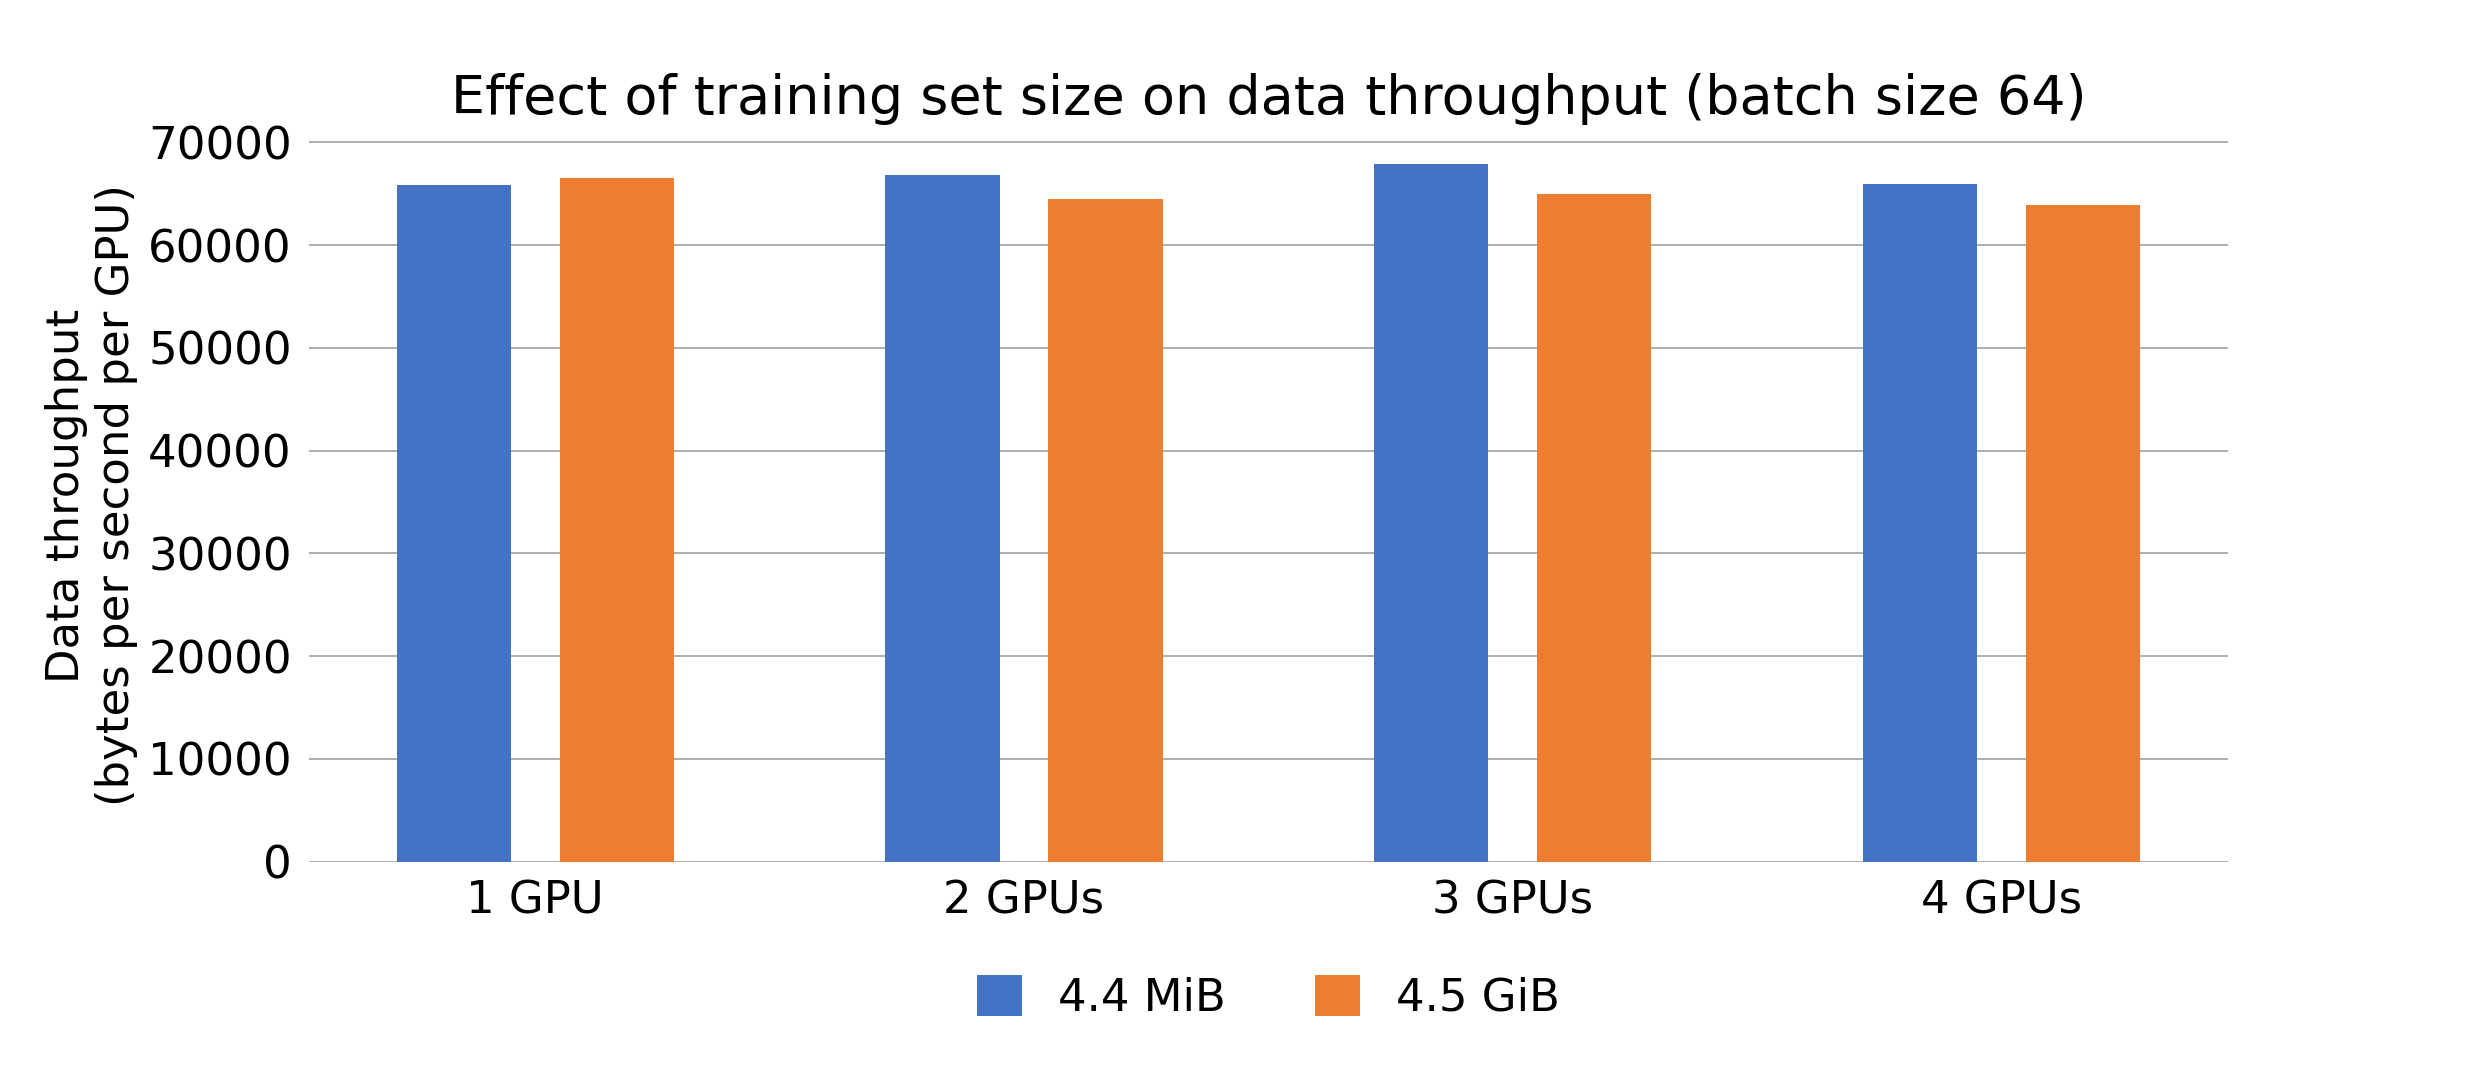
\includegraphics[width=1.0\textwidth,keepaspectratio]{4_1_1.png}
\end{frame}

\begin{frame}{Larger Datasets}
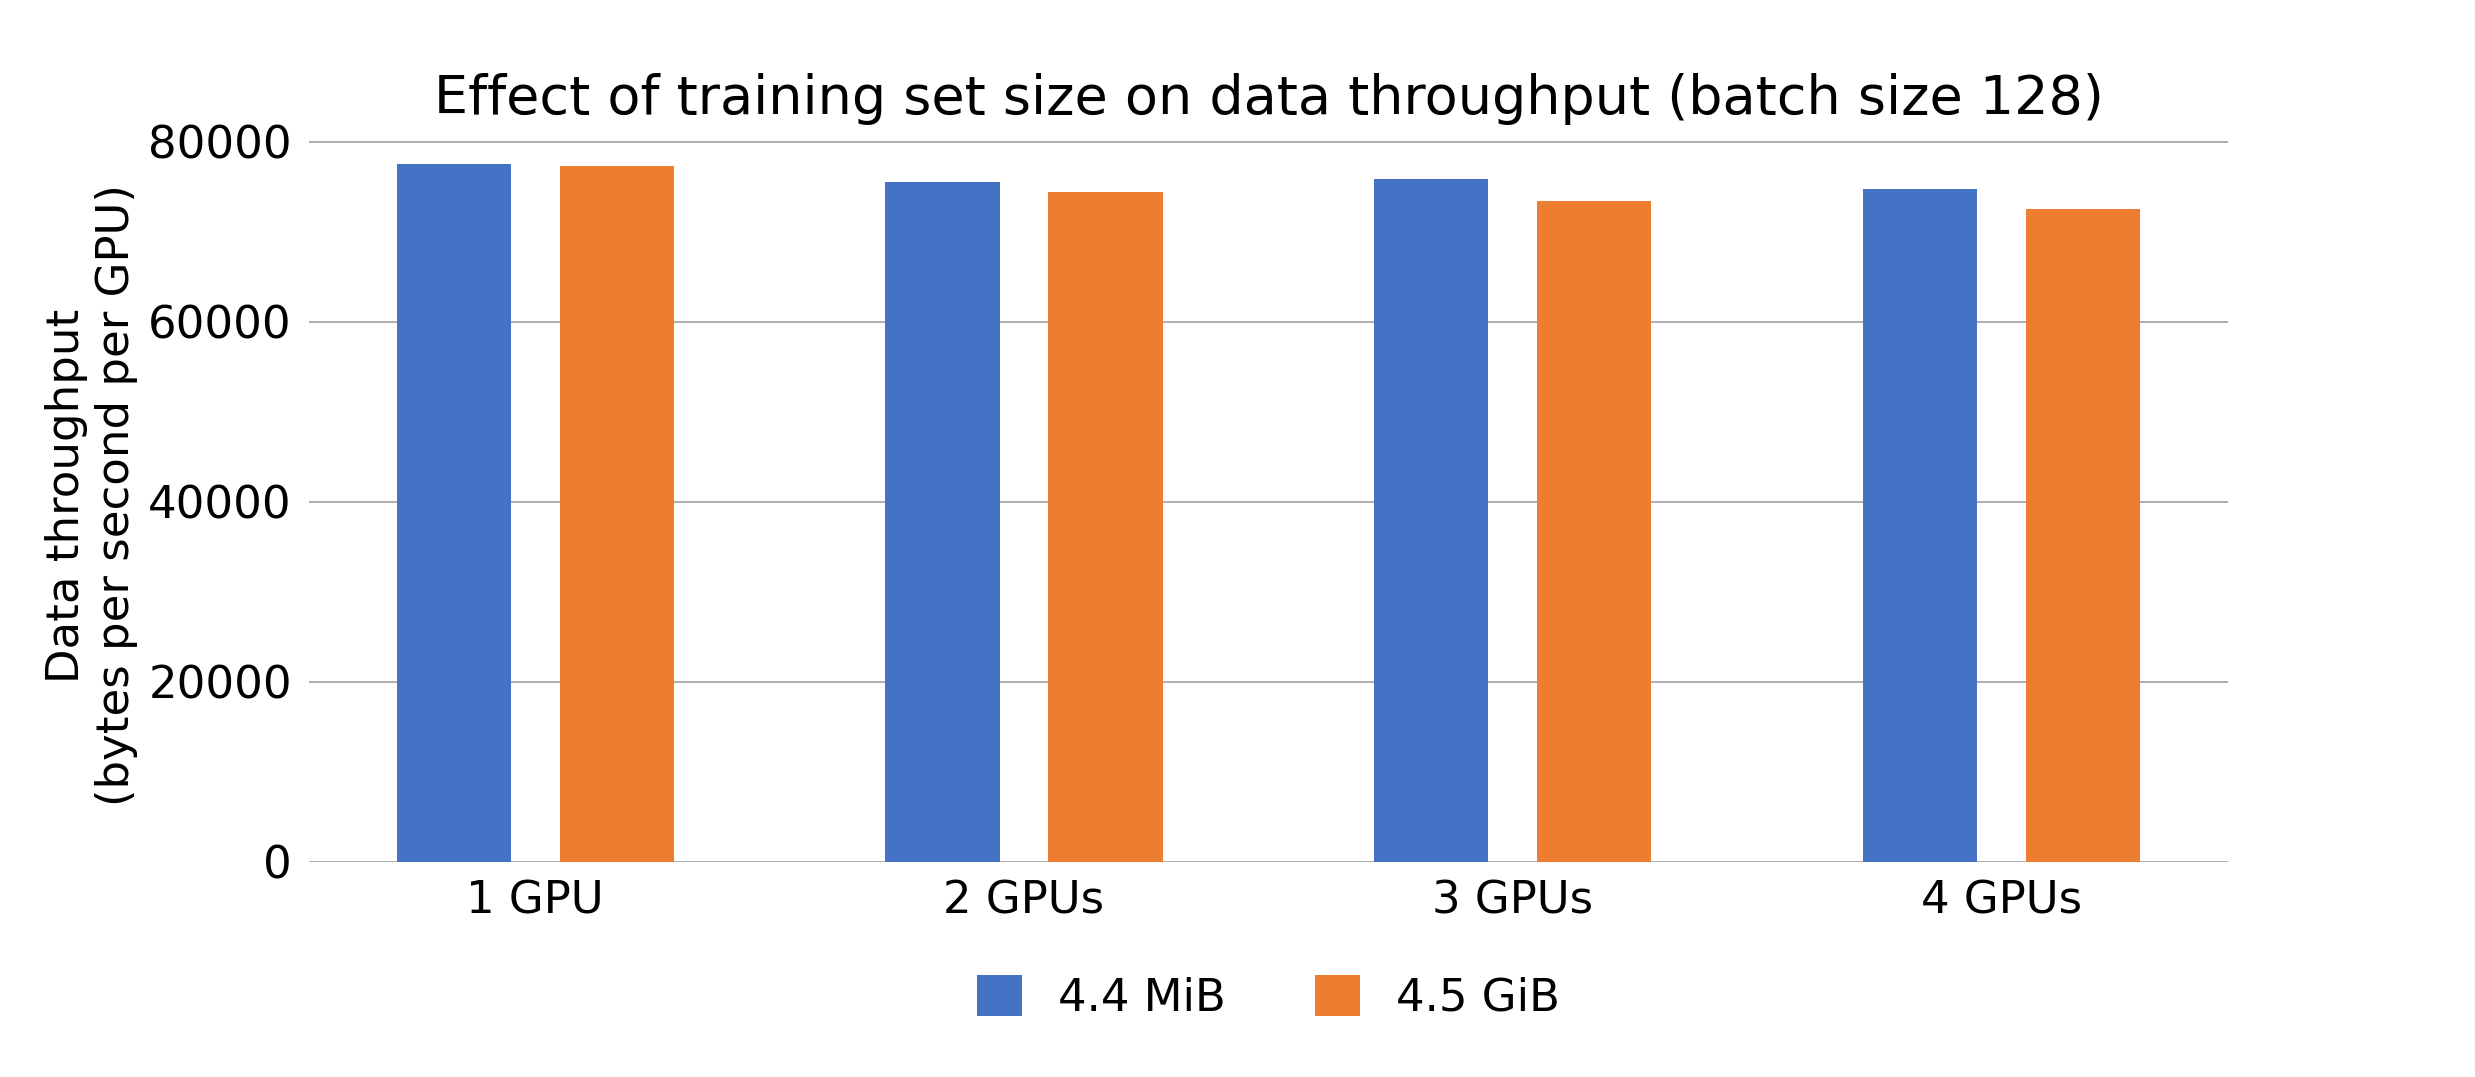
\includegraphics[width=1.0\textwidth,keepaspectratio]{4_1_2.png}
\end{frame}

\begin{frame}{Larger Datasets}
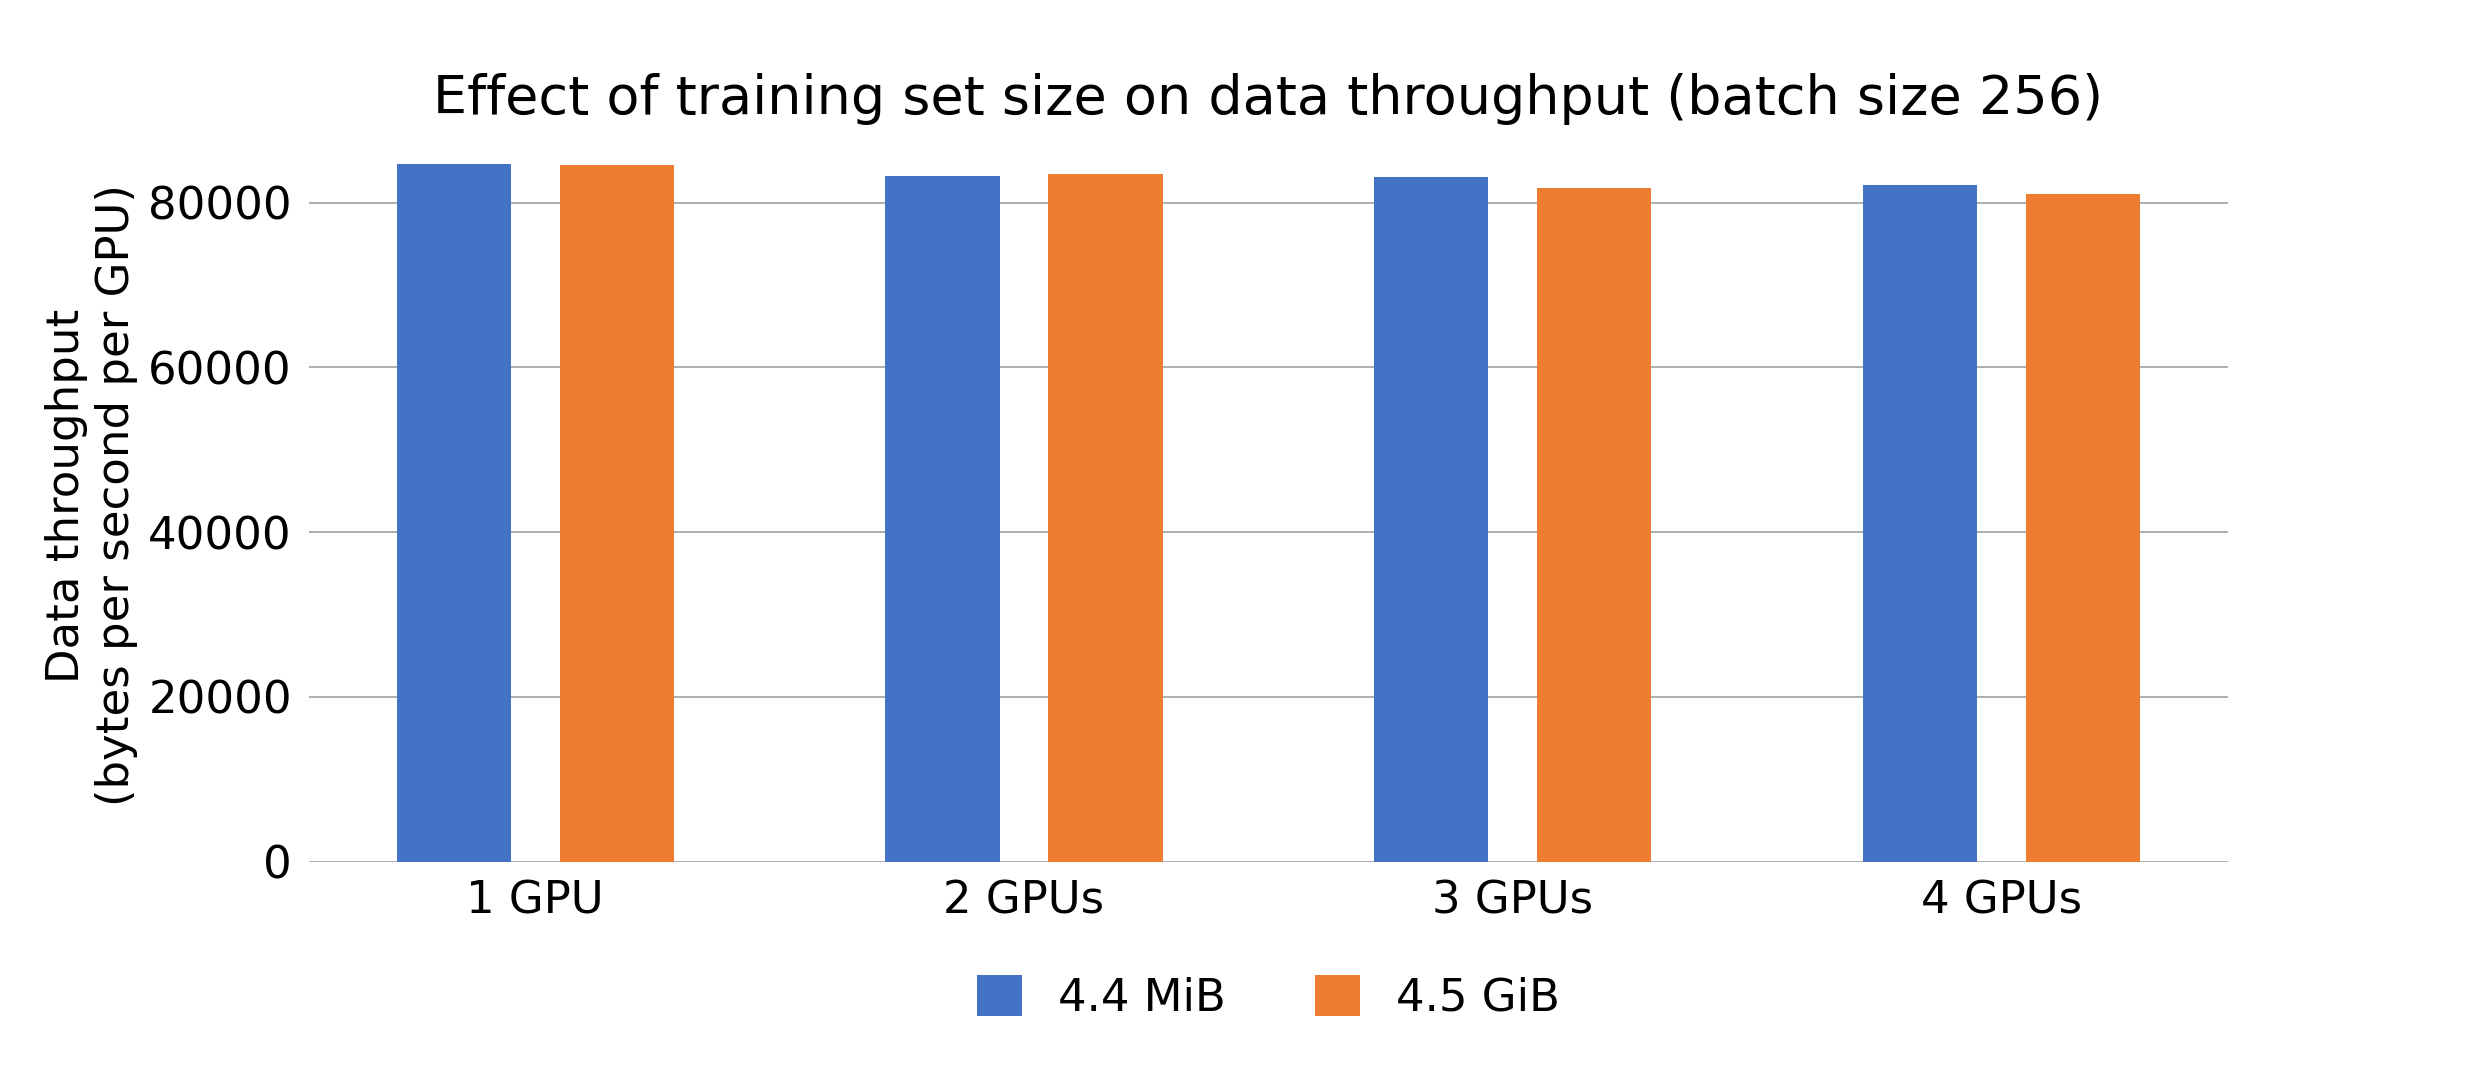
\includegraphics[width=1.0\textwidth,keepaspectratio]{4_1_3.png}
\end{frame}

\begin{frame}{Larger Datasets - Observations}

\begin{enumerate}
  \item Average epoch time scales only slightly more than linearly with training dataset size.
  \item Batch size has a larger impact on data throughput than dataset size.
  \item Throughput reducing slightly as the number of GPUs increases.
  \item PCI data sent and received remains broadly the same for both the small and large training datasets.
  \item Rule of thumb: training time increases linearly with training data size.
\end{enumerate}

\end{frame}

% Section divider slide
\section{Model Parallelism}

\begin{frame}{Model Parallelism}
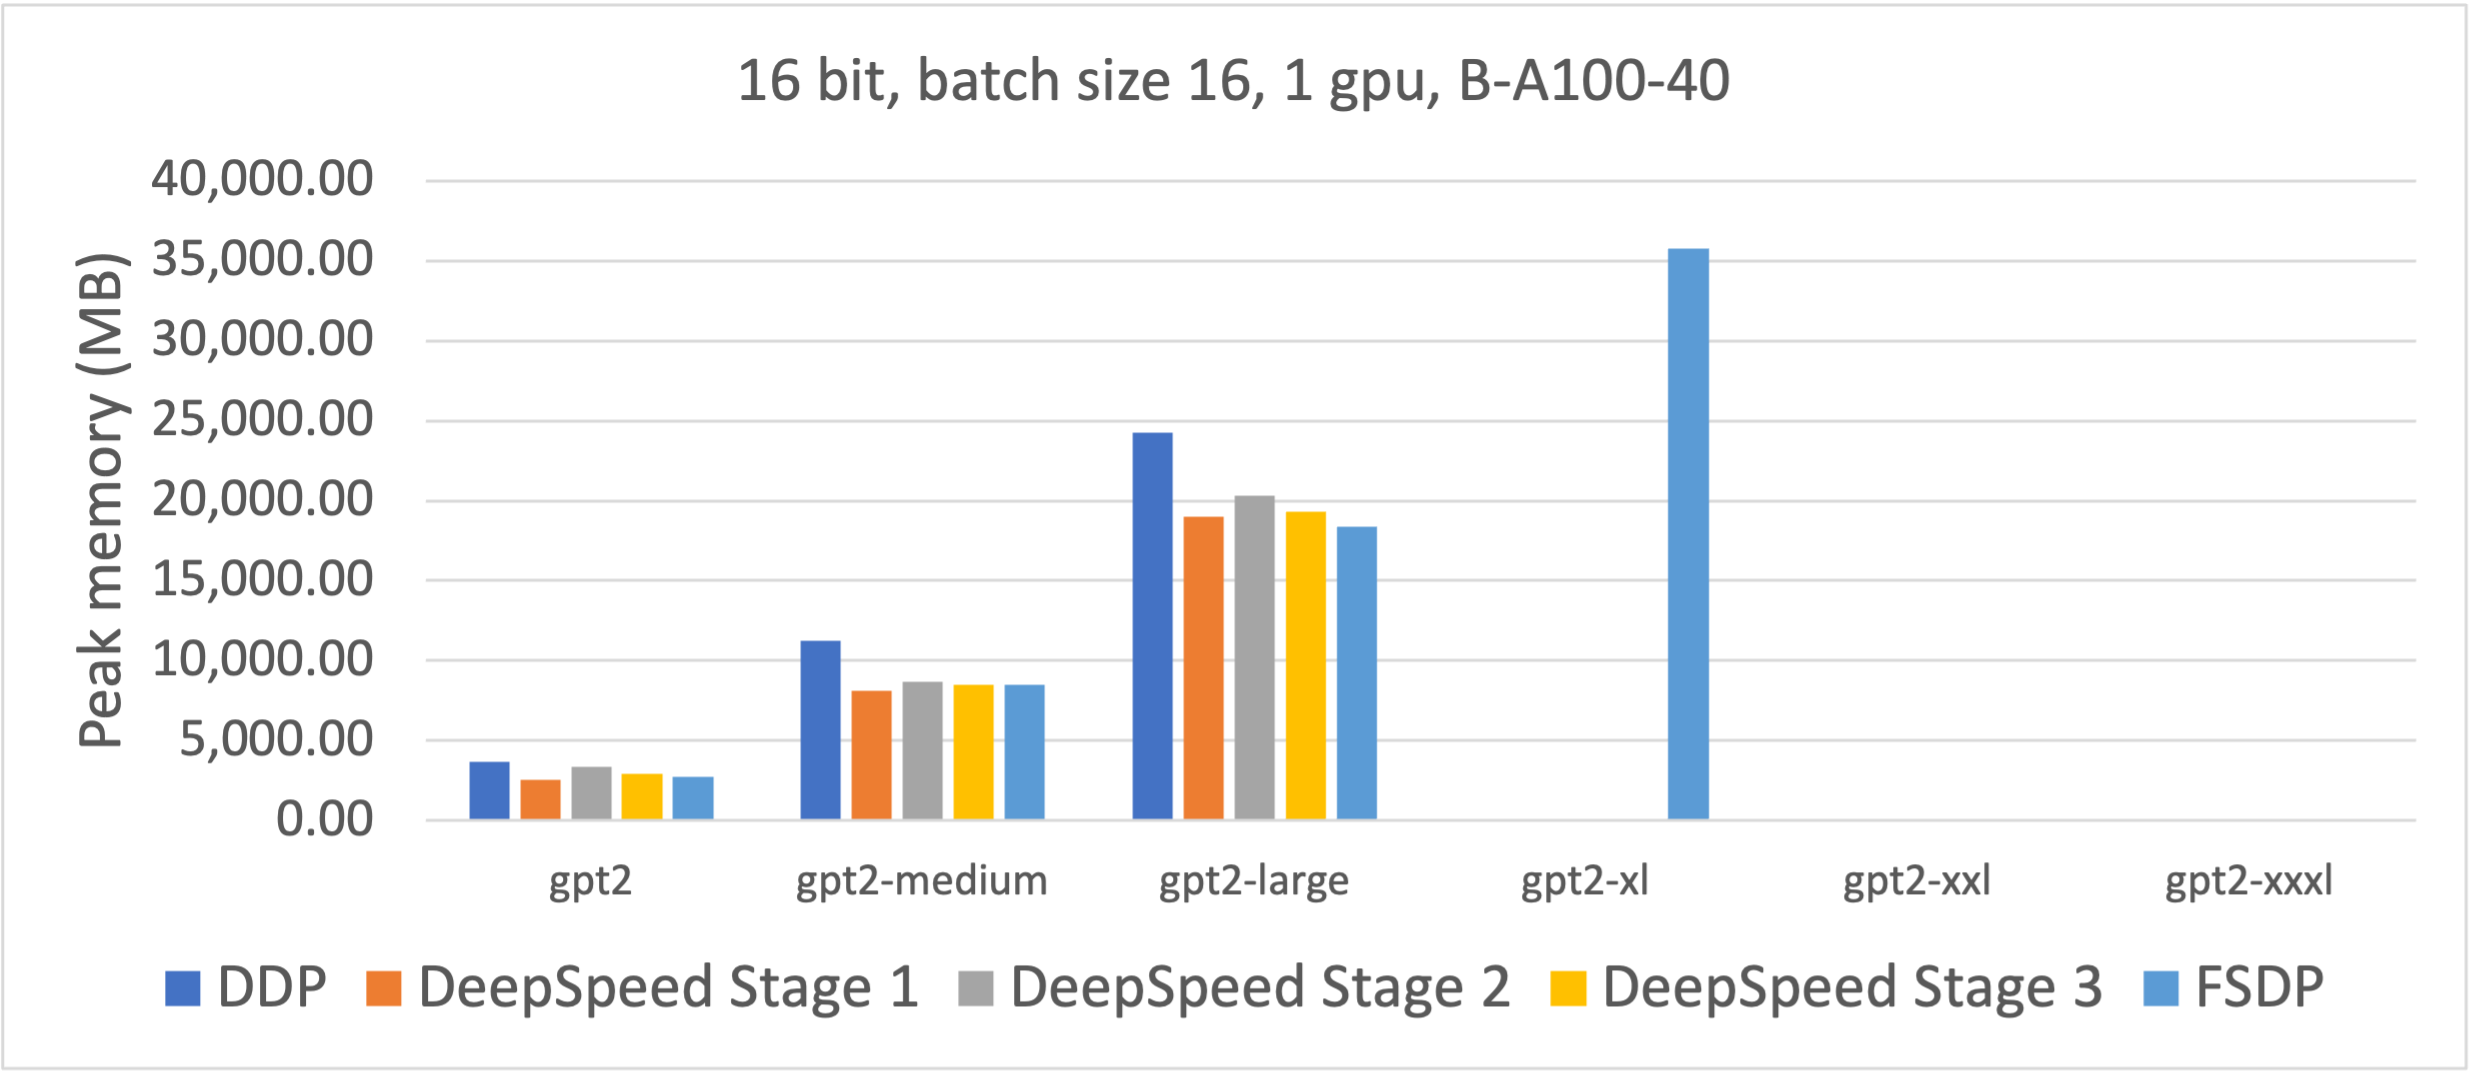
\includegraphics[width=1.0\textwidth,keepaspectratio]{5_1_1.png}
\end{frame}

\begin{frame}{Model Parallelism}
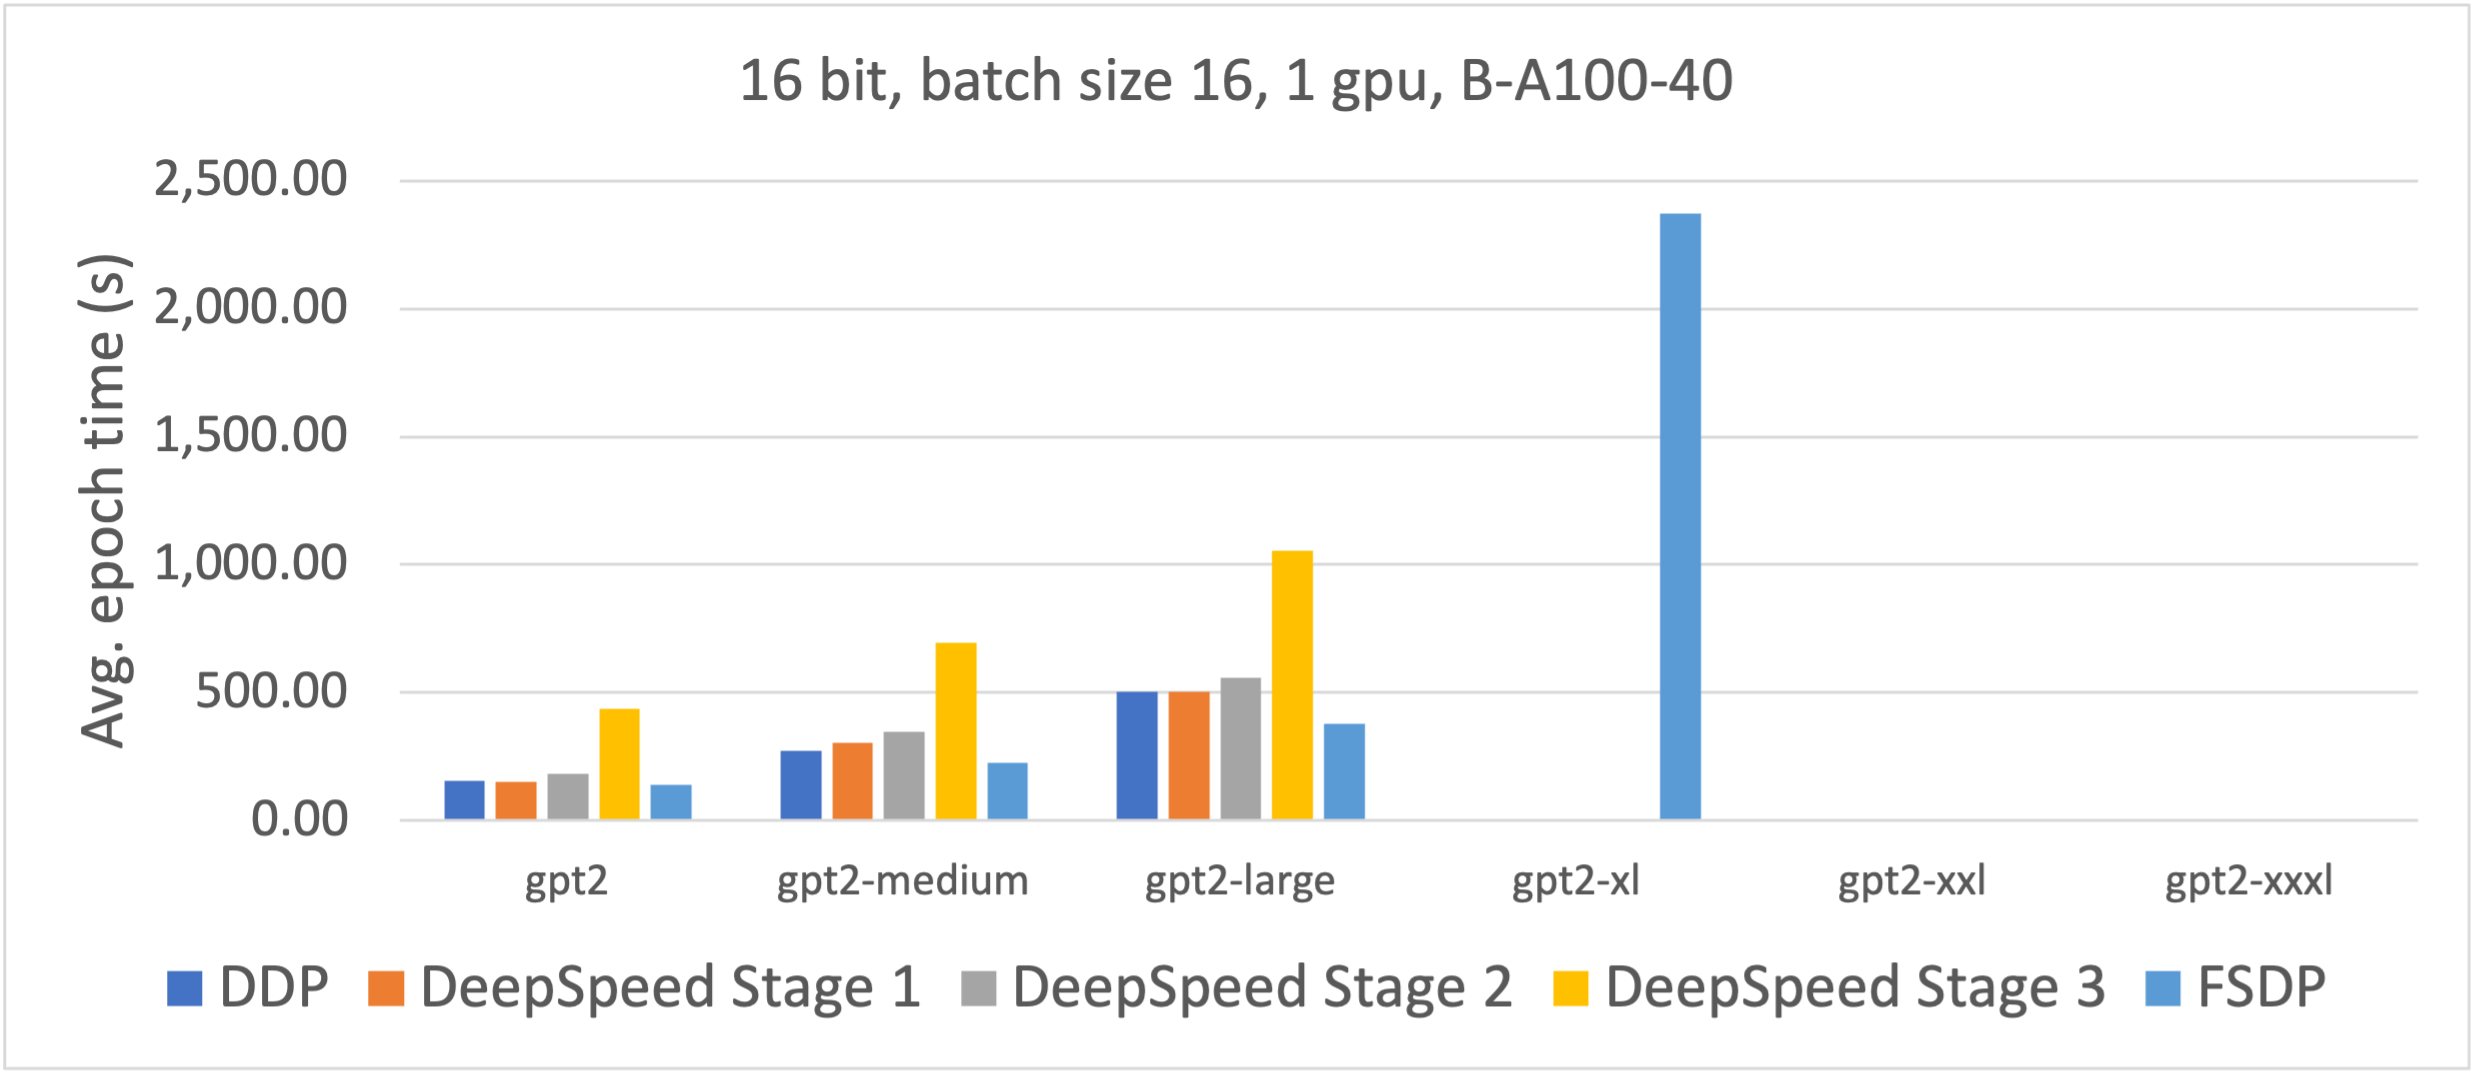
\includegraphics[width=1.0\textwidth,keepaspectratio]{5_1_2.png}
\end{frame}

\begin{frame}{Model Parallelism}
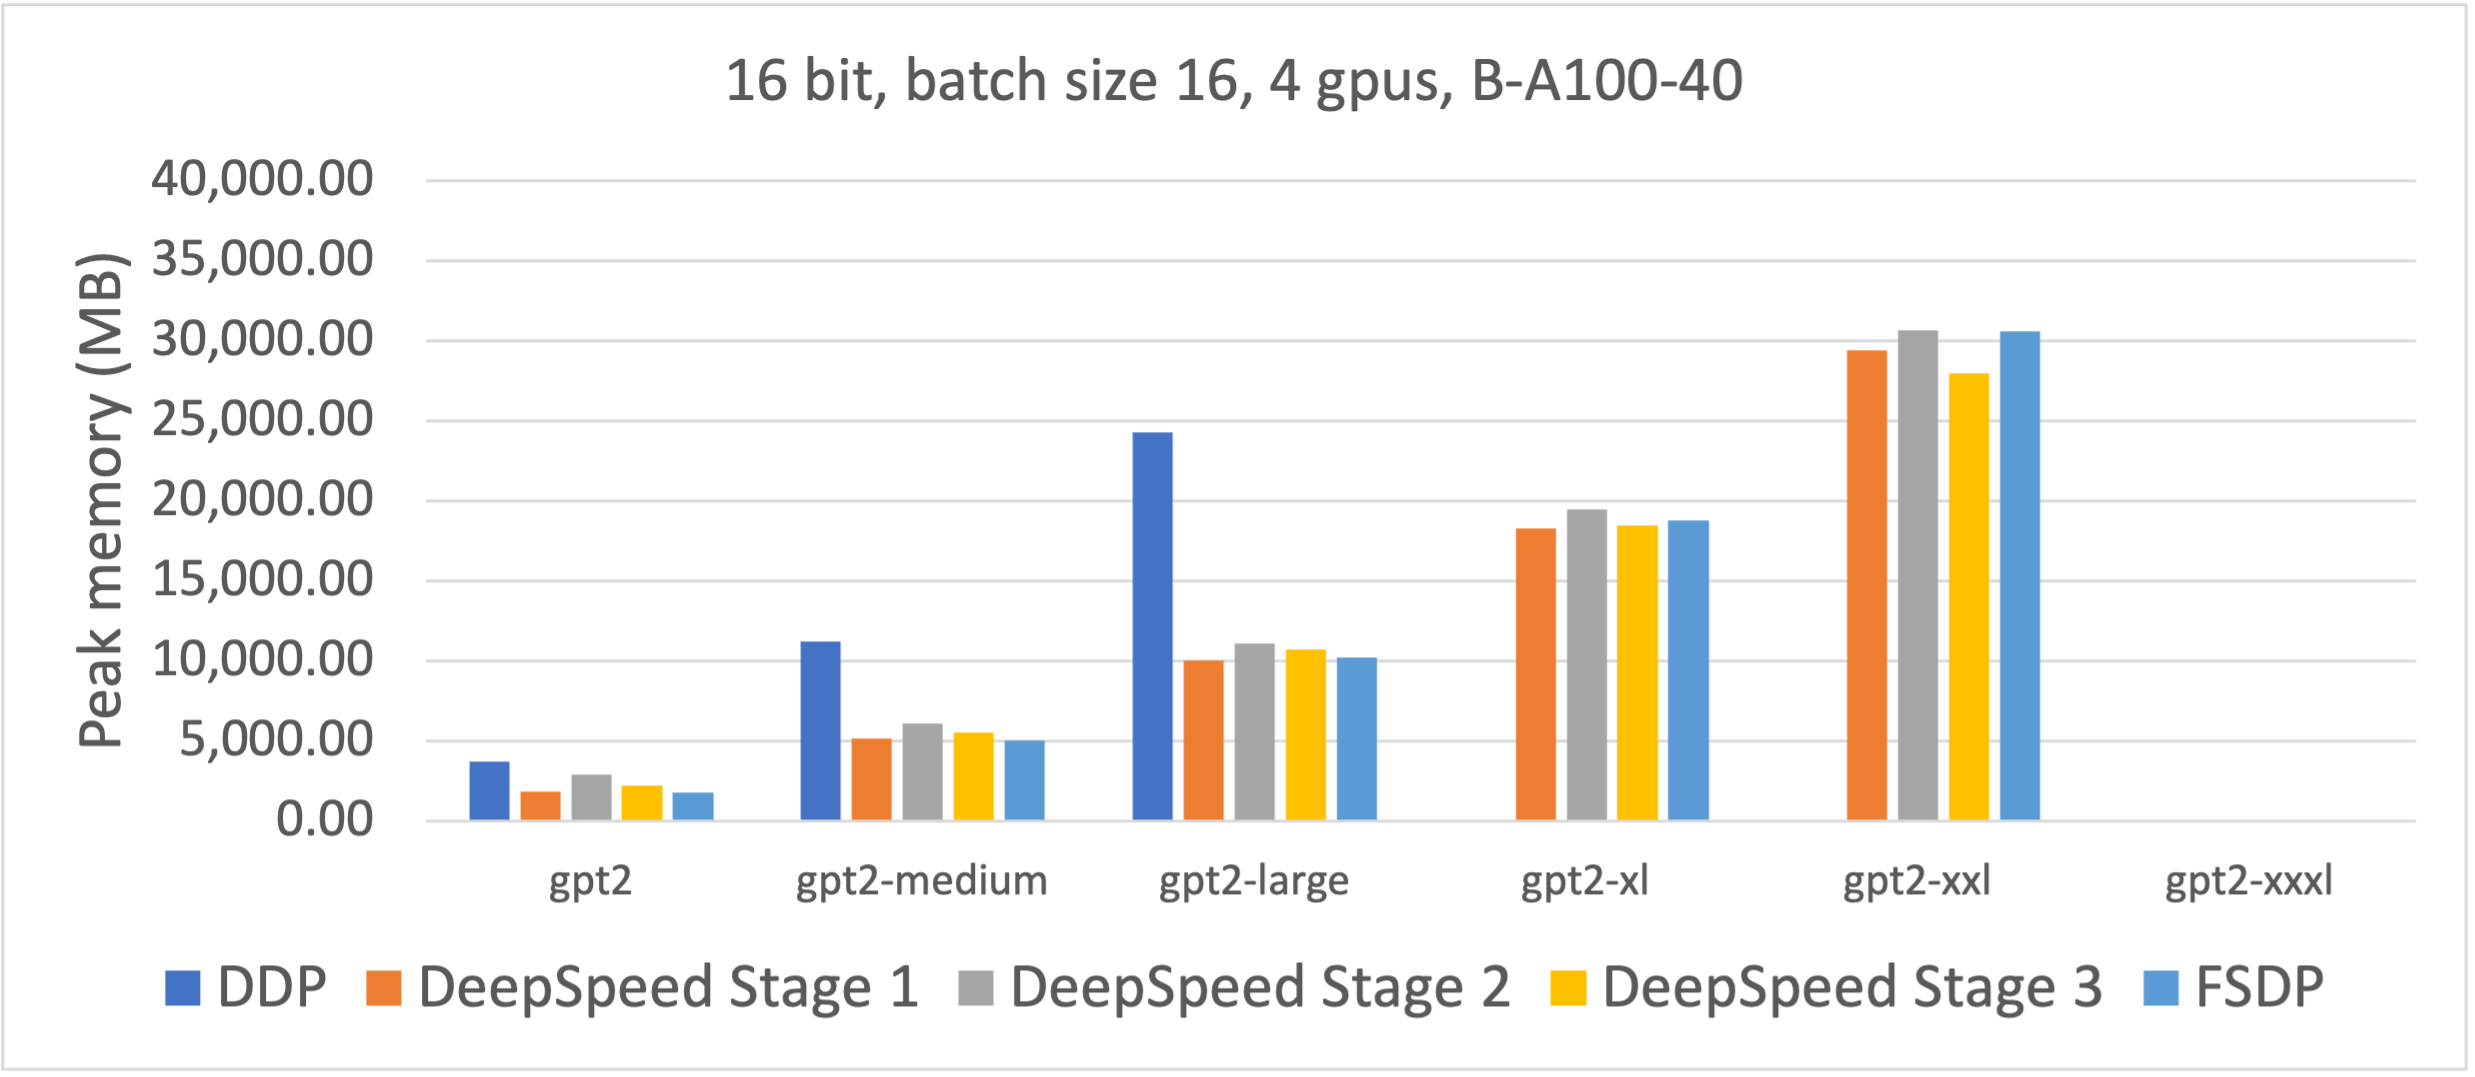
\includegraphics[width=1.0\textwidth,keepaspectratio]{5_2_1.png}
\end{frame}

\begin{frame}{Model Parallelism}
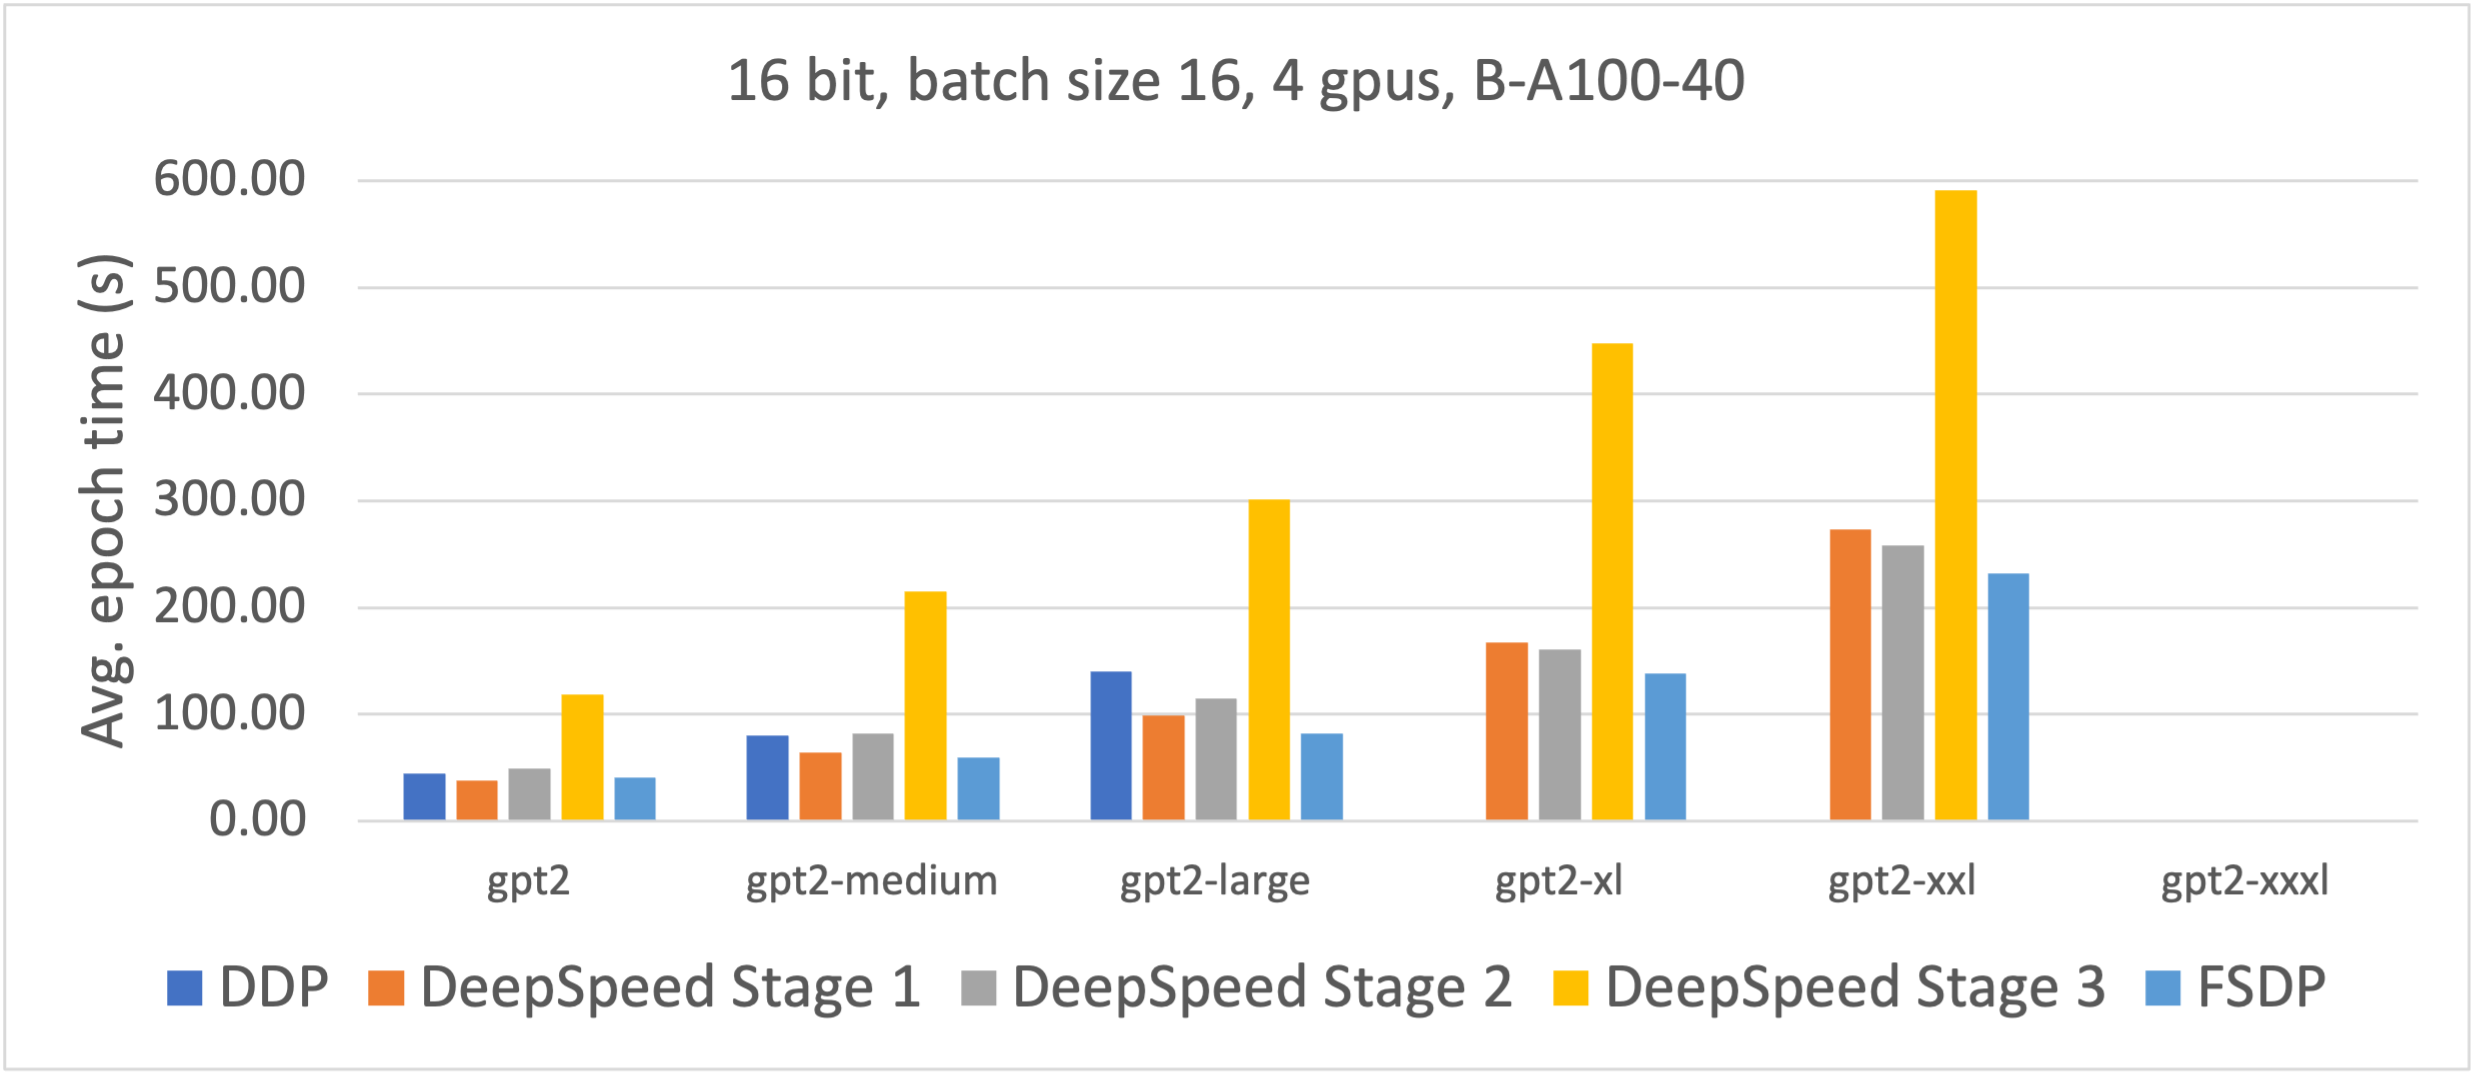
\includegraphics[width=1.0\textwidth,keepaspectratio]{5_2_2.png}
\end{frame}

\begin{frame}{Model Parallelism}
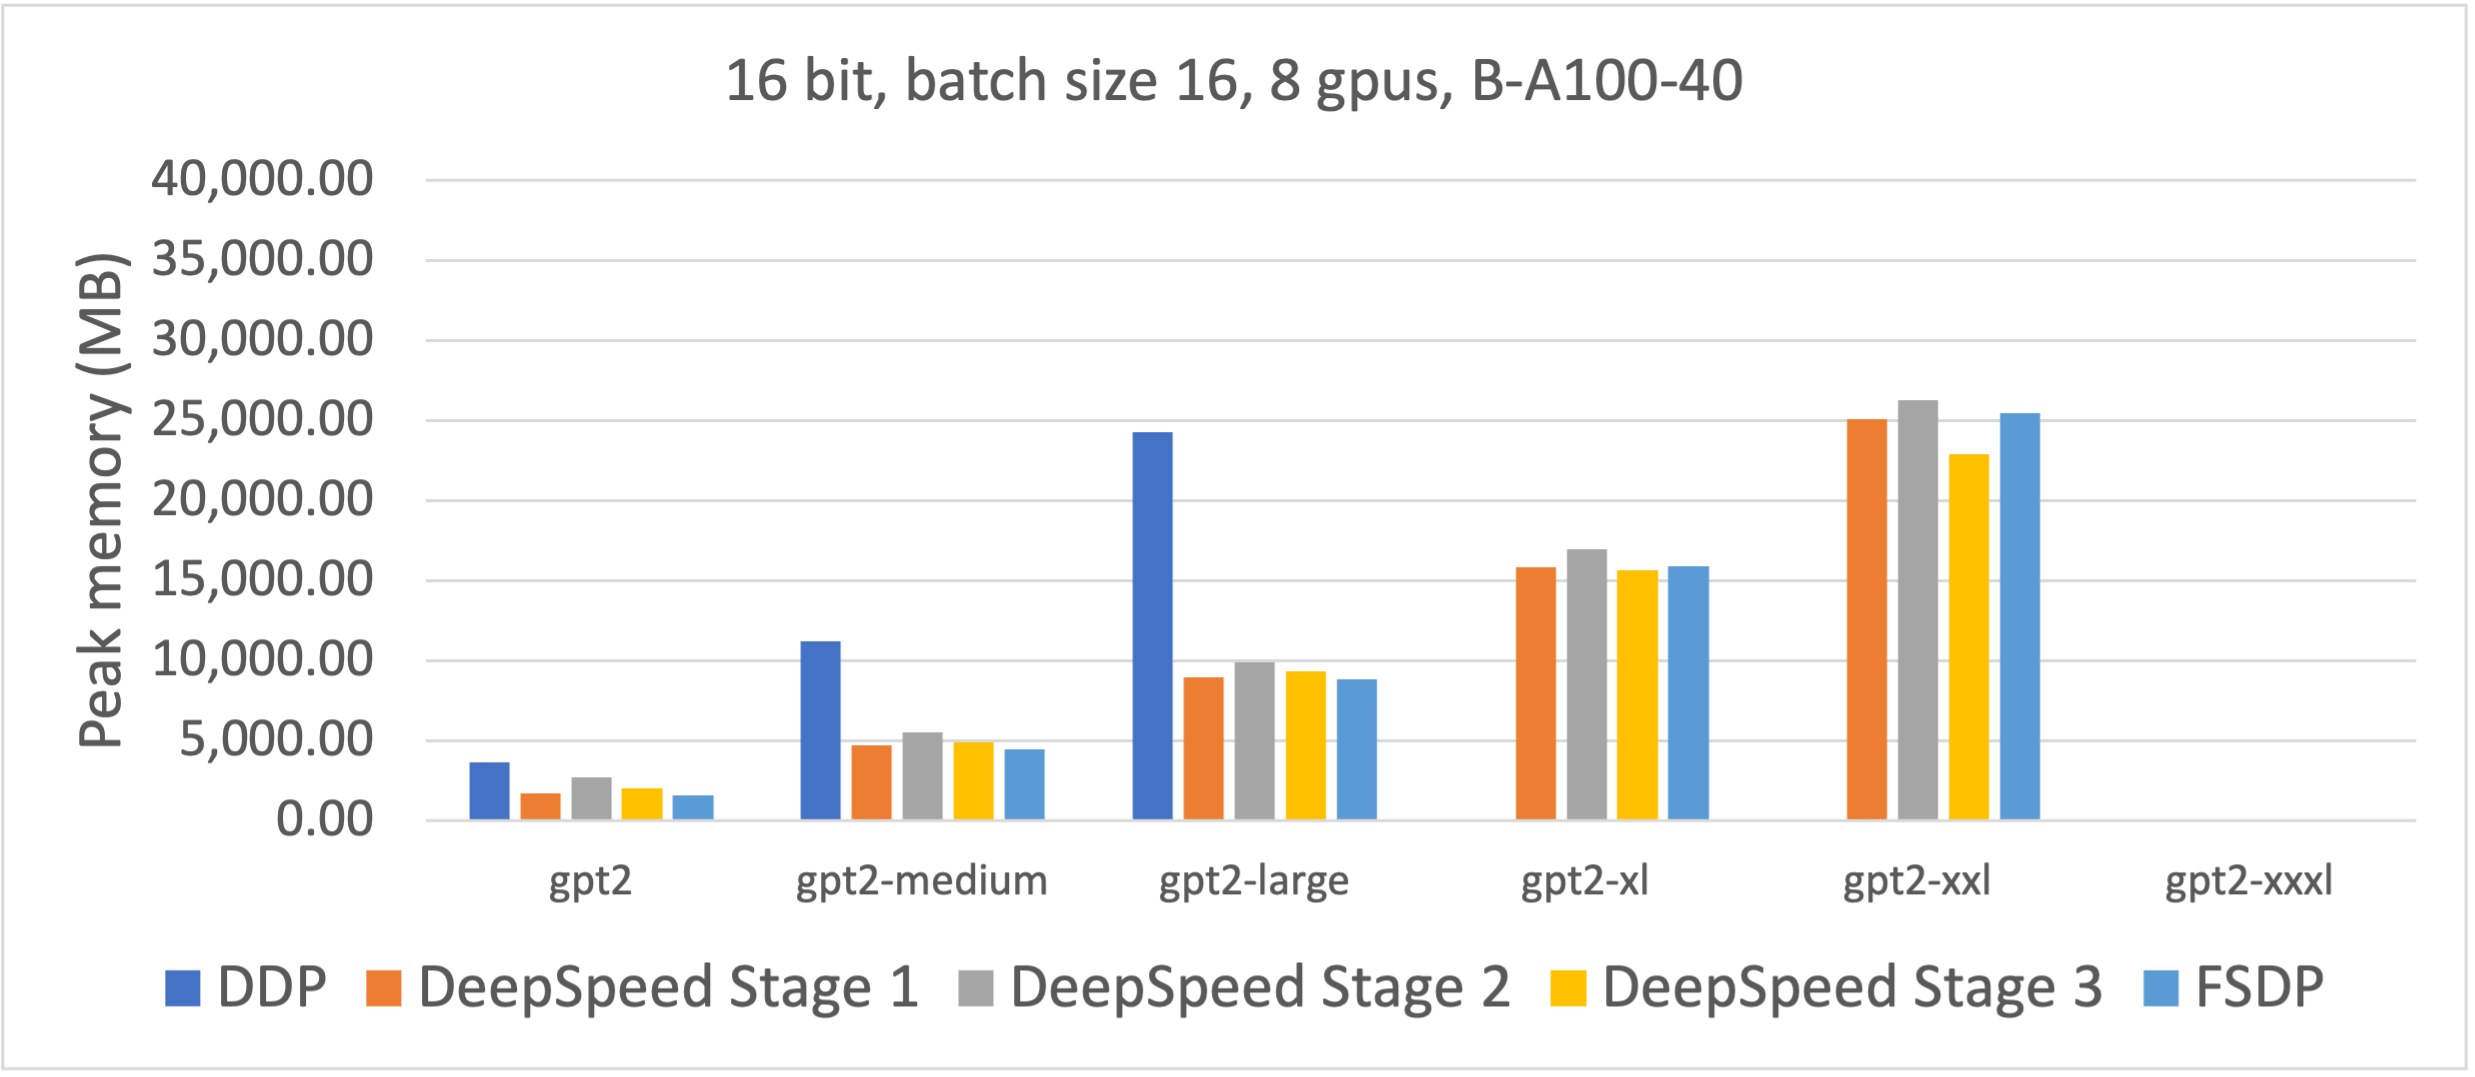
\includegraphics[width=1.0\textwidth,keepaspectratio]{5_3_1.png}
\end{frame}

\begin{frame}{Model Parallelism}
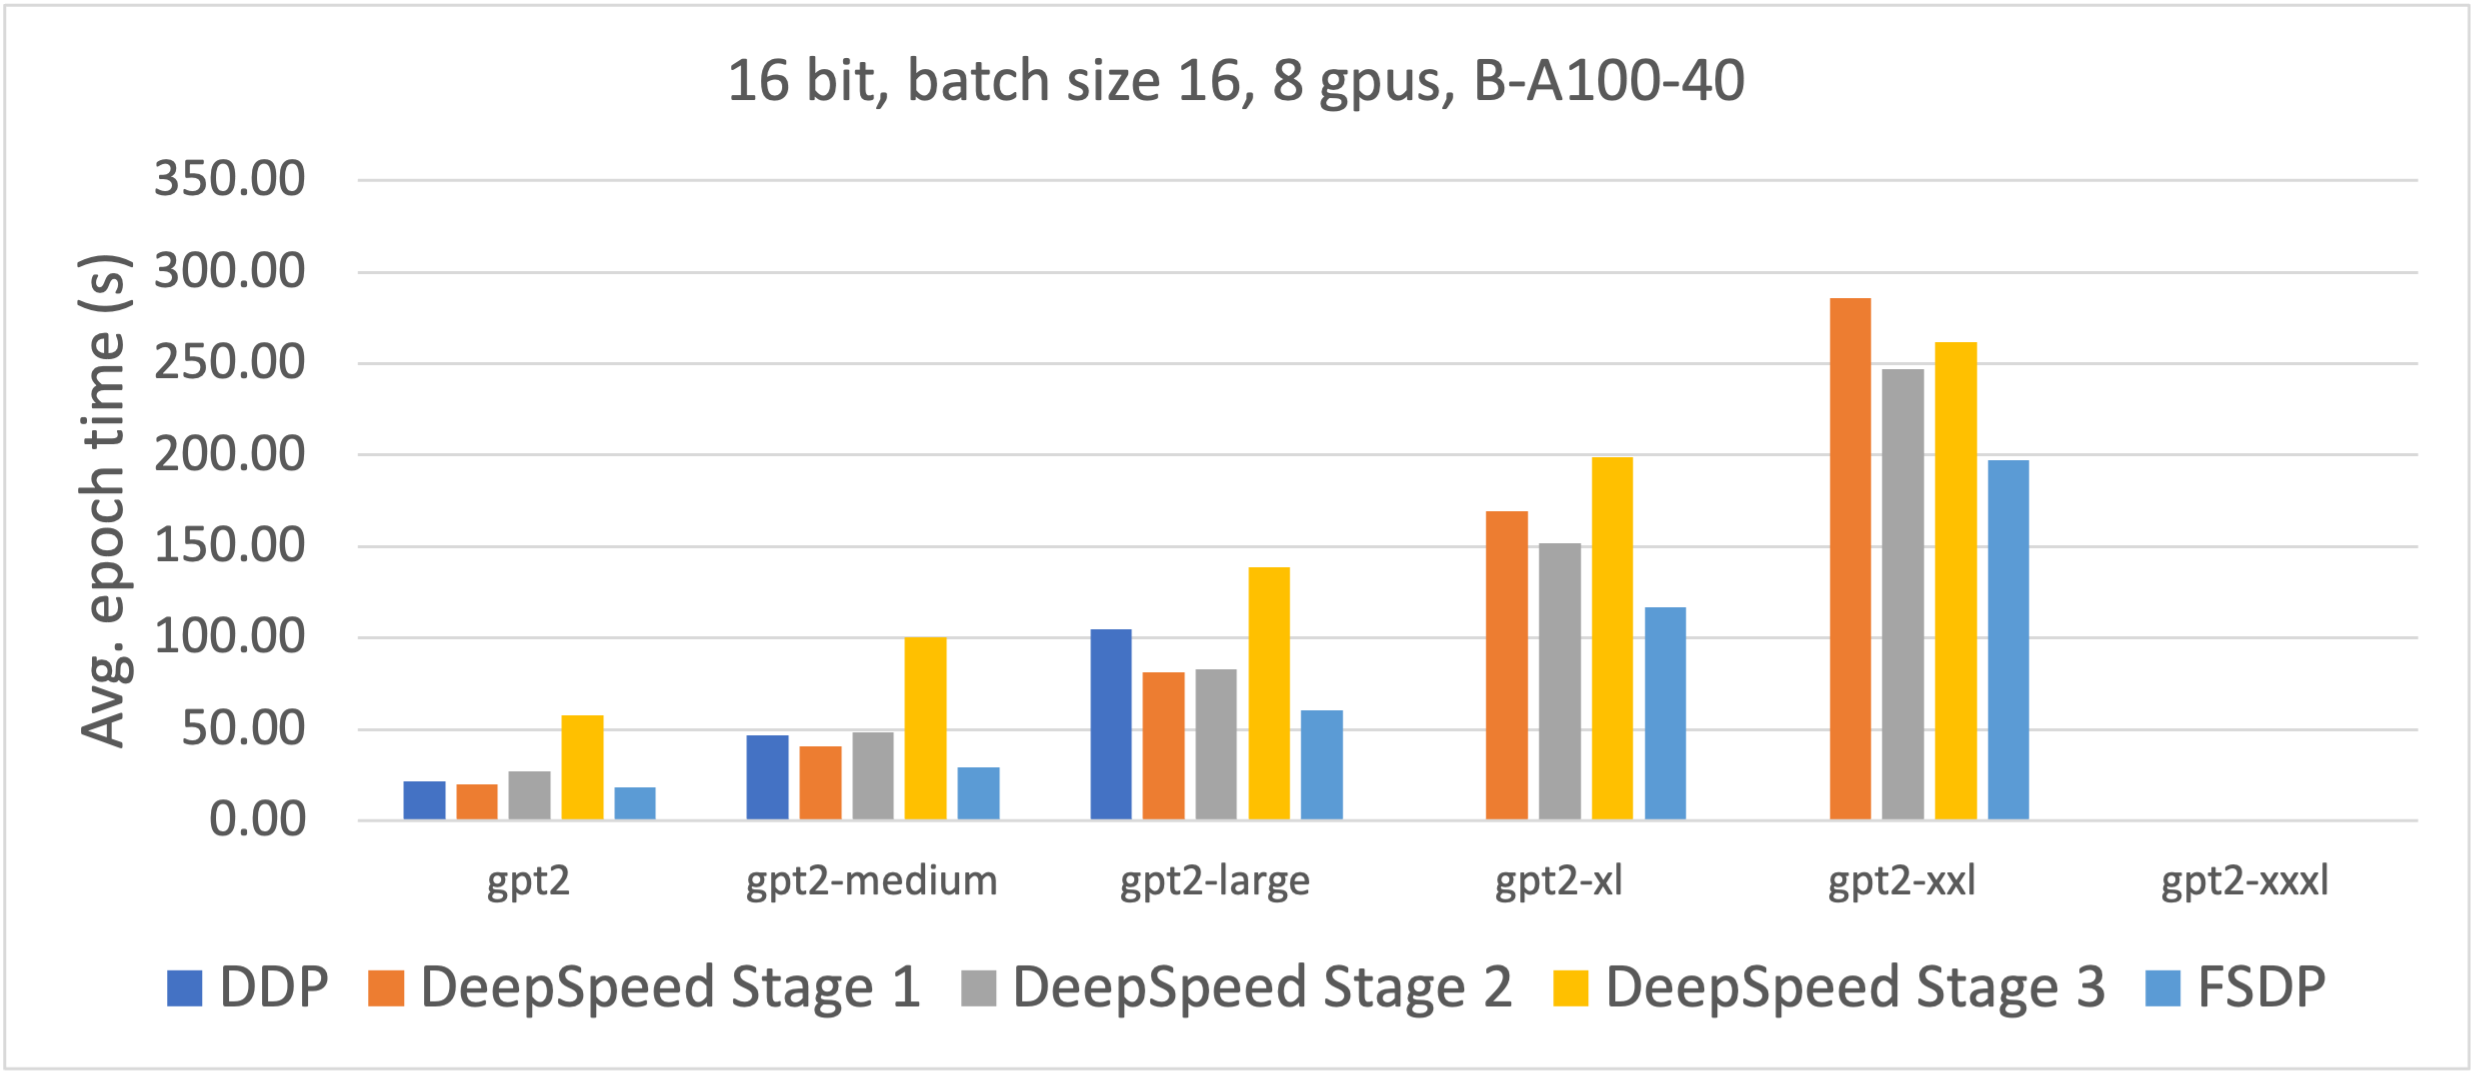
\includegraphics[width=1.0\textwidth,keepaspectratio]{5_3_2.png}
\end{frame}

\begin{frame}{Model Parallelism}
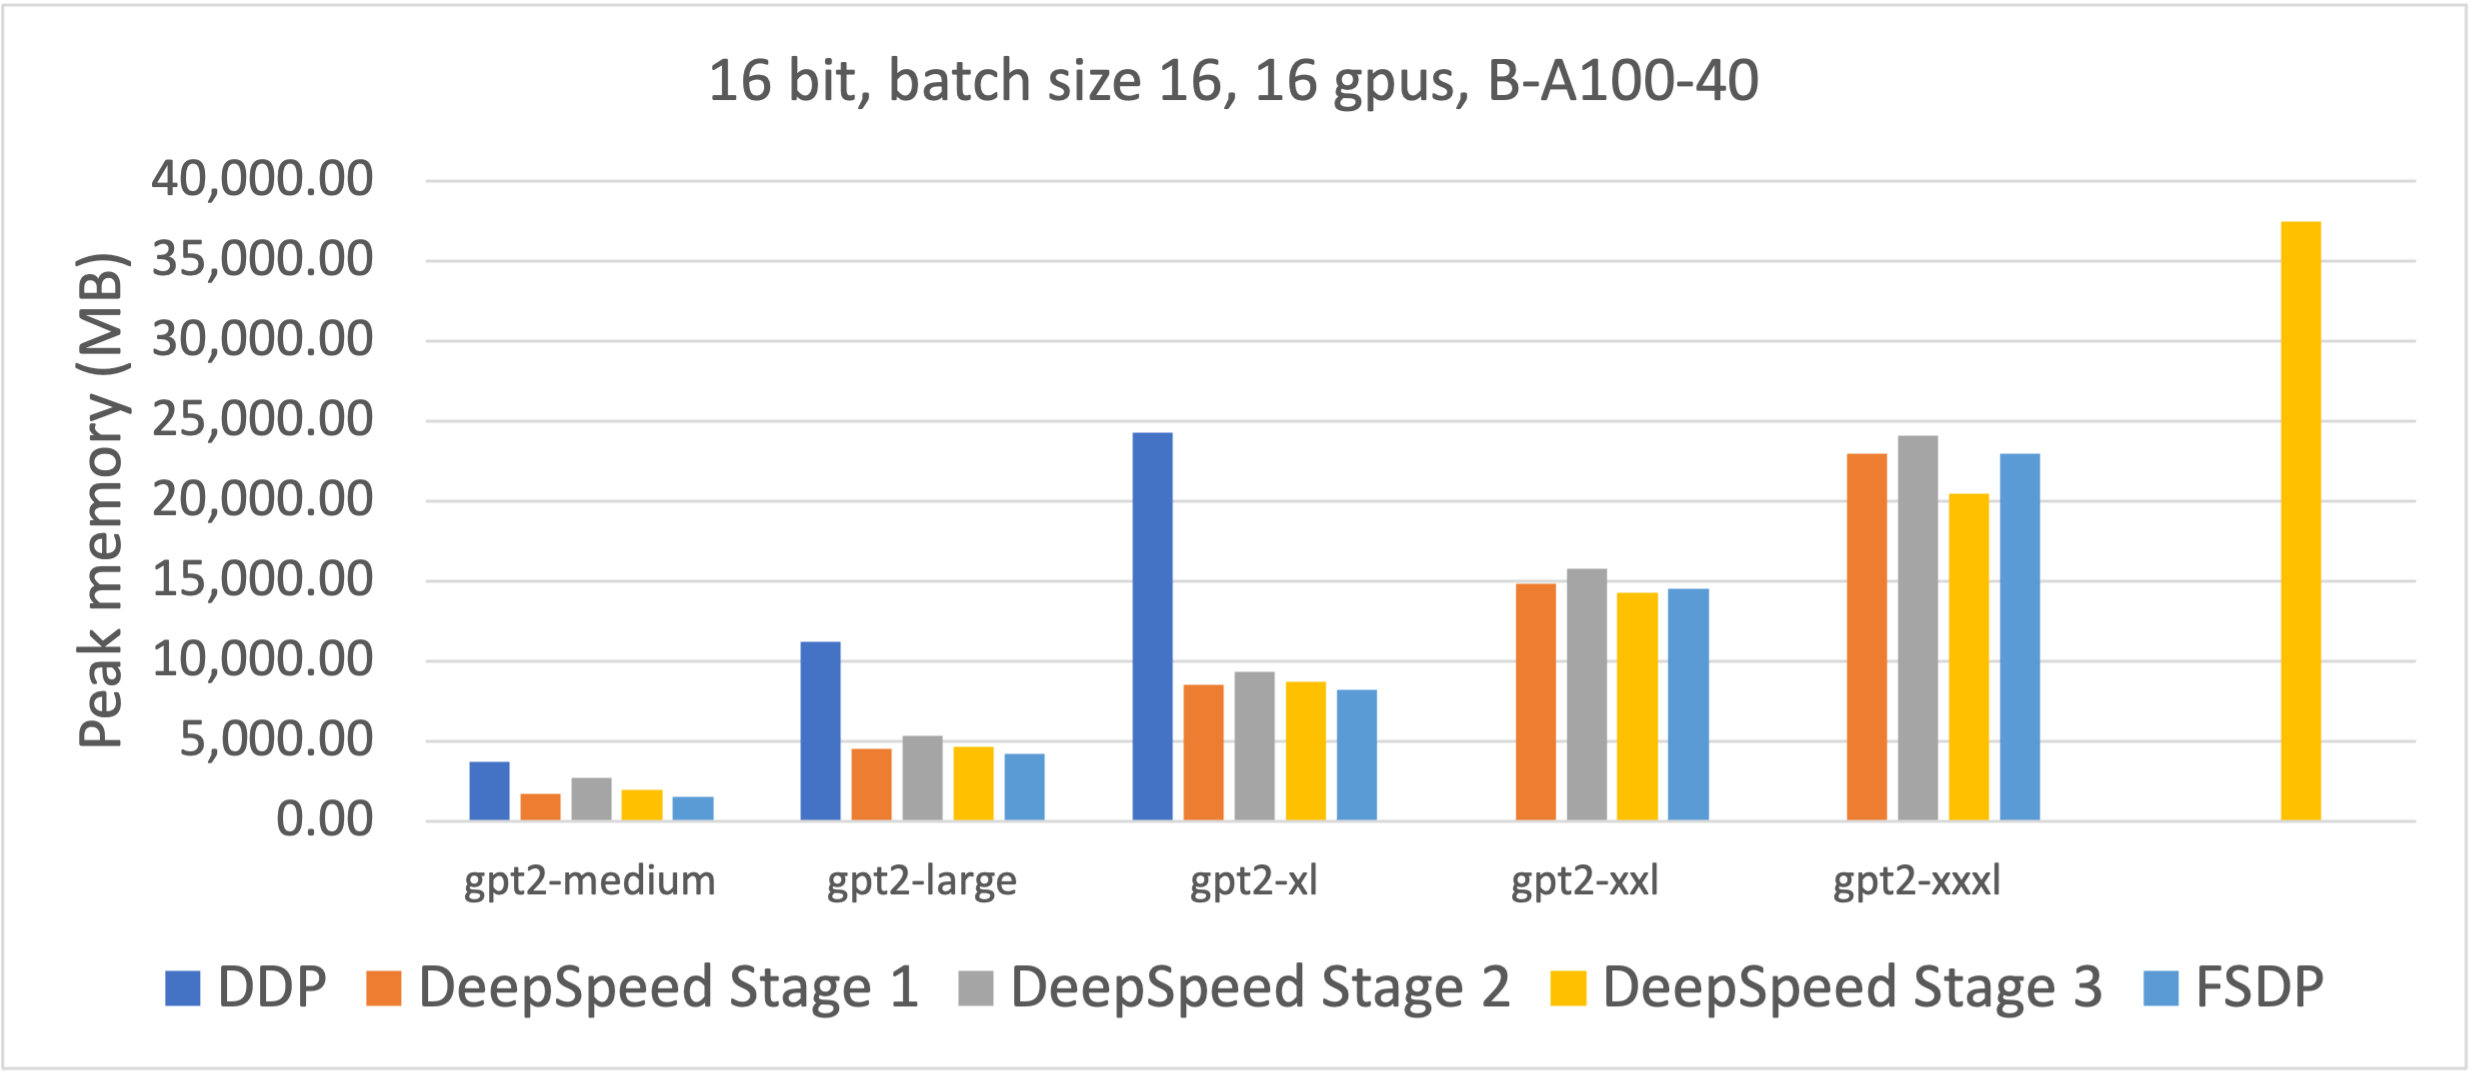
\includegraphics[width=1.0\textwidth,keepaspectratio]{5_4_1.png}
\end{frame}

\begin{frame}{Model Parallelism}
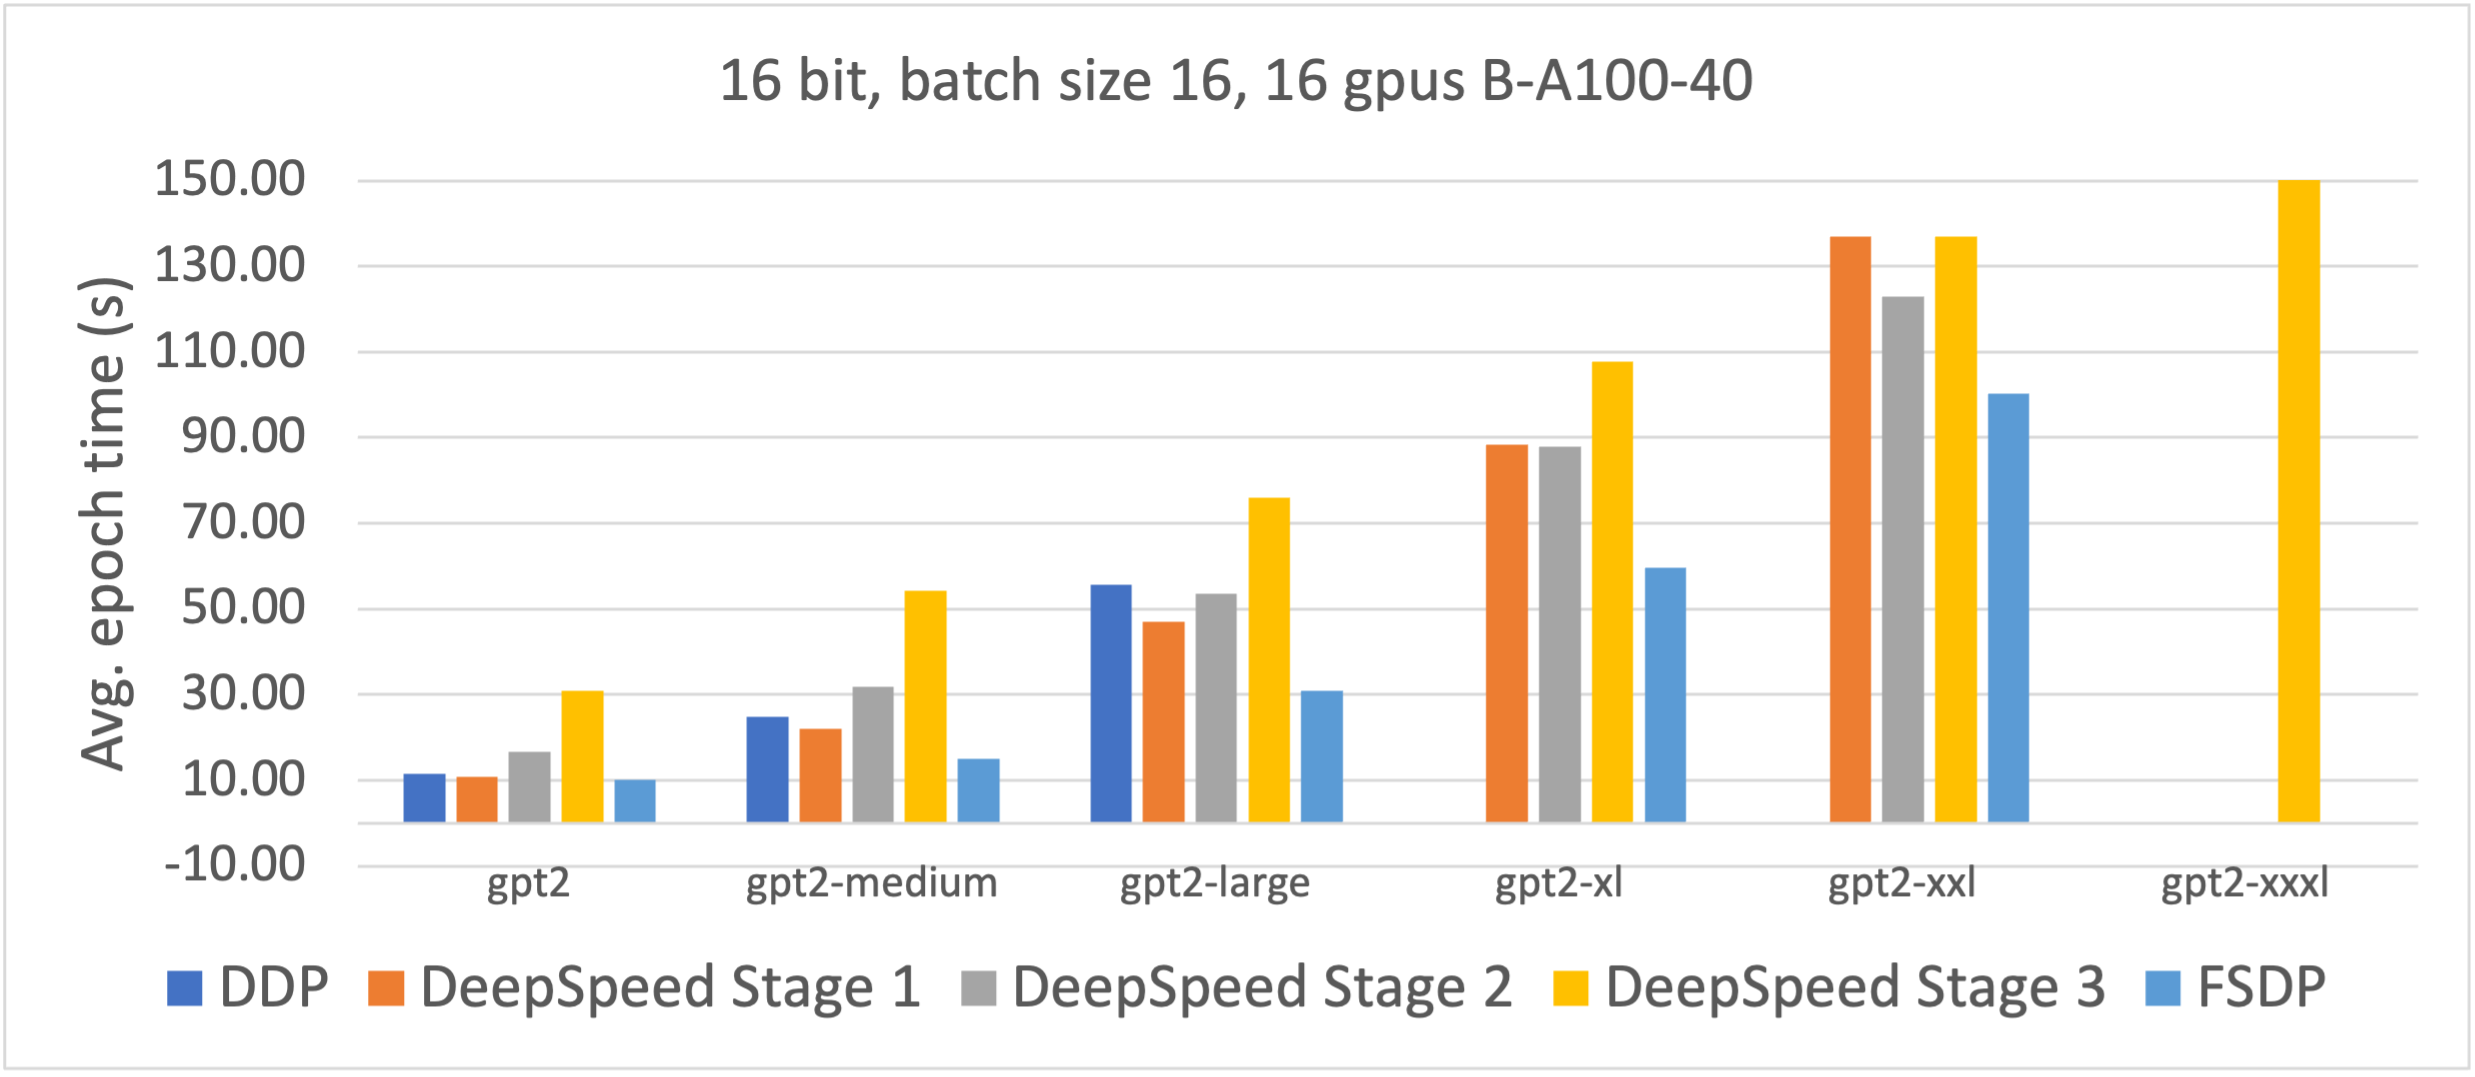
\includegraphics[width=1.0\textwidth,keepaspectratio]{5_4_2.png}
\end{frame}

\begin{frame}{Model Parallelism}
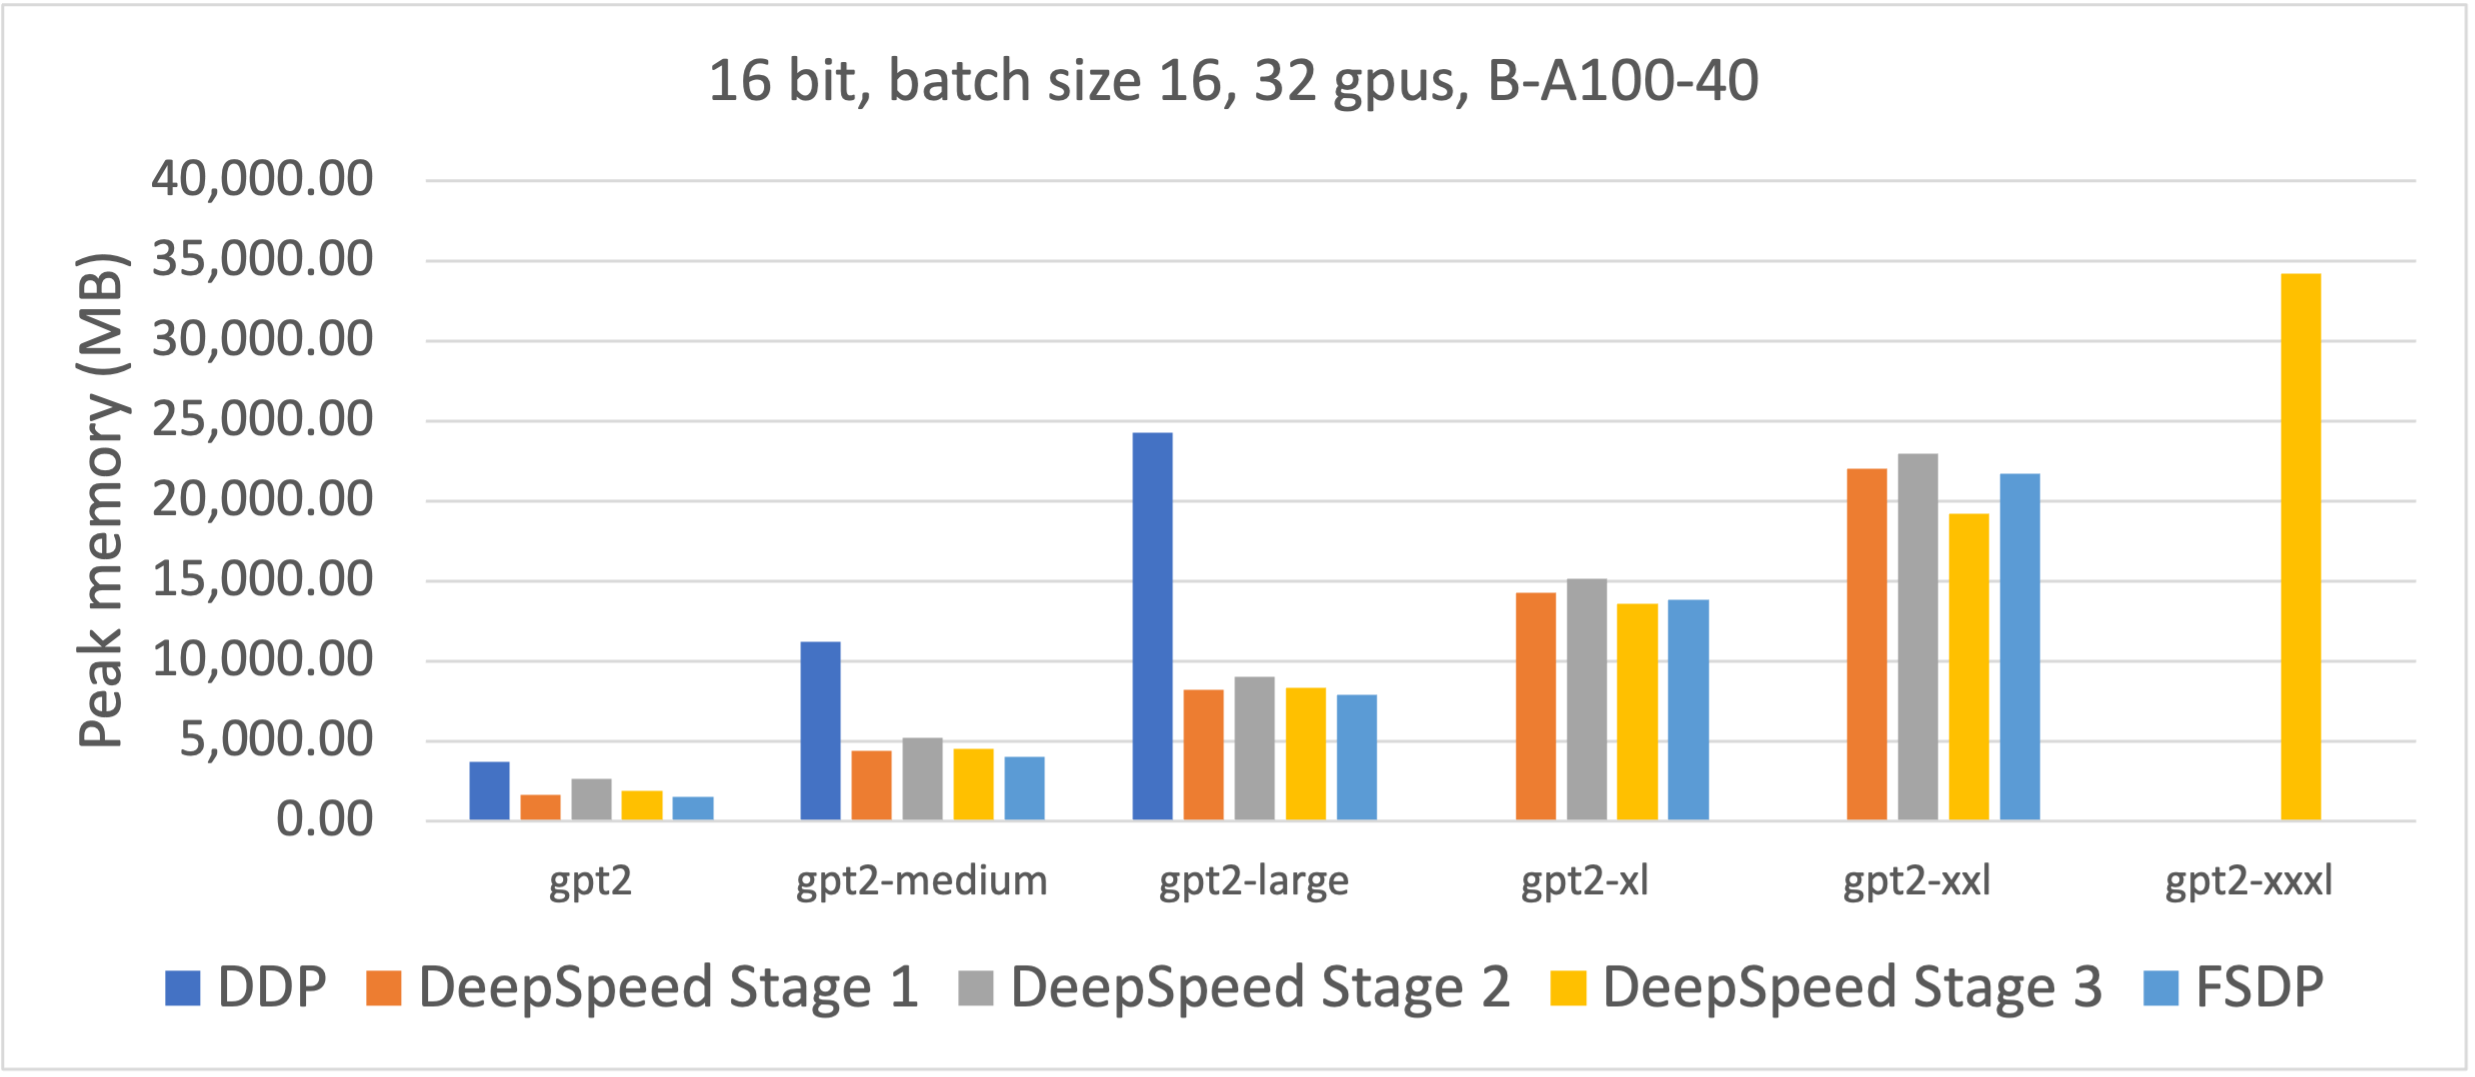
\includegraphics[width=1.0\textwidth,keepaspectratio]{5_5_1.png}
\end{frame}

\begin{frame}{Model Parallelism}
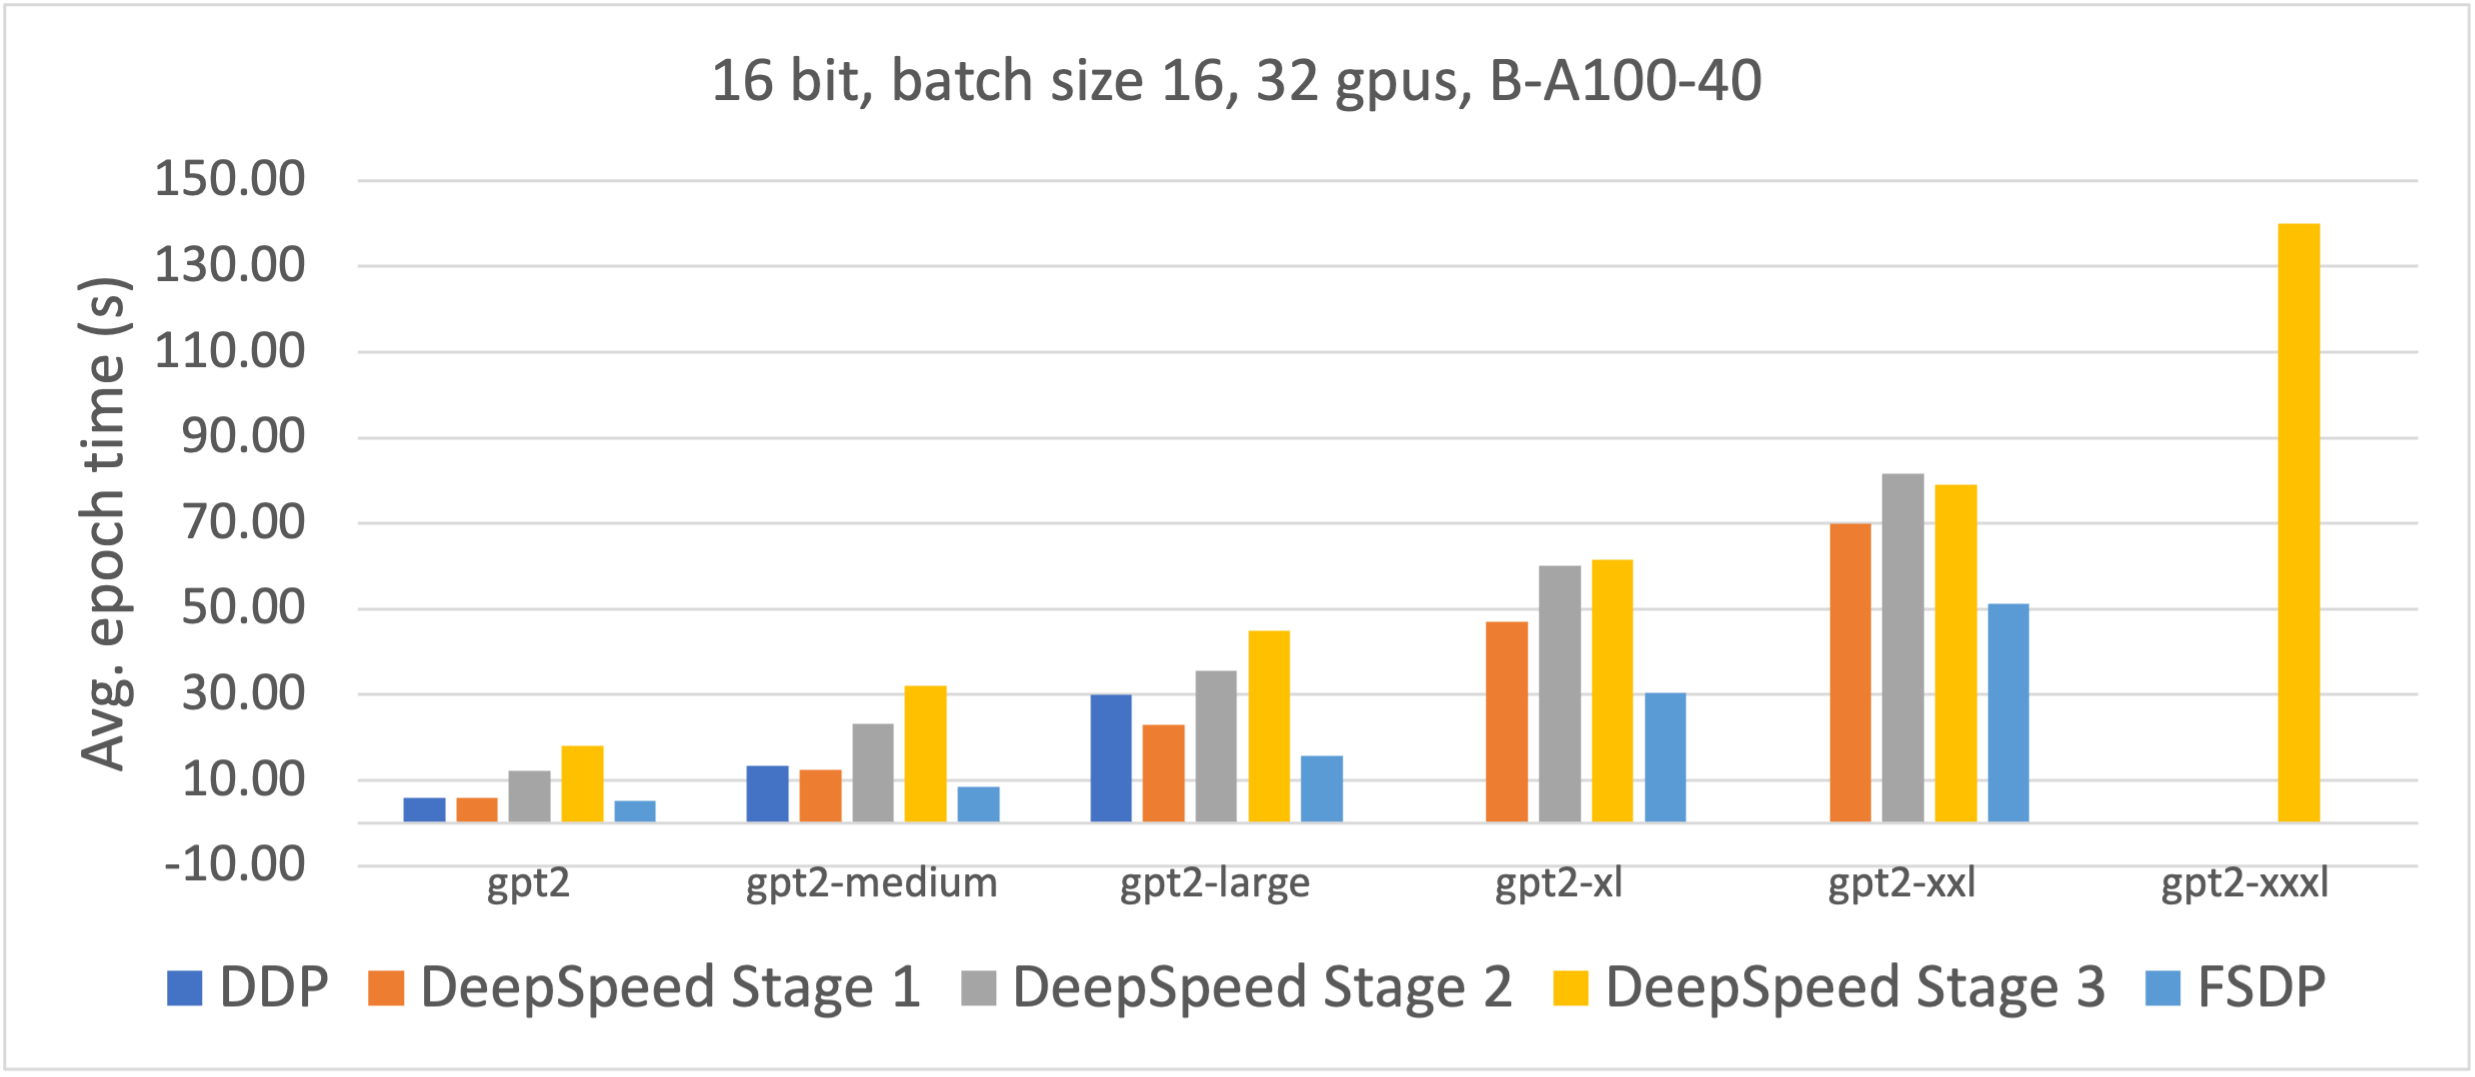
\includegraphics[width=1.0\textwidth,keepaspectratio]{5_5_2.png}
\end{frame}

\begin{frame}{Model Parallelism - Observations}

\begin{enumerate}
  \item Utilising DeepSpeed Stage 3 enables training of the largest model size with a minimum of 16 GPUs.
  \item FSDP facilitates training GPT2-XXL when at least 4 GPUs are utilised.
  \item With 1 GPU, DeepSpeed and FSDP used less memory than DDP.
  \item With 4 GPUs DeepSpeed and FSDP used 50\% less memory than DDP.
  \item Similar trends were found for 8, 16, and 32 GPUs.
  \item With more than 8 GPUs, DeepSpeed Stage 3 exhibited lowest average peak memory for model sizes of GPT2-XL or larger.
\end{enumerate}

\end{frame}

% Section divider slide
\section{Graphcore IPU-IPOD 16}

\begin{frame}{Graphcore IPU-IPOD 16}
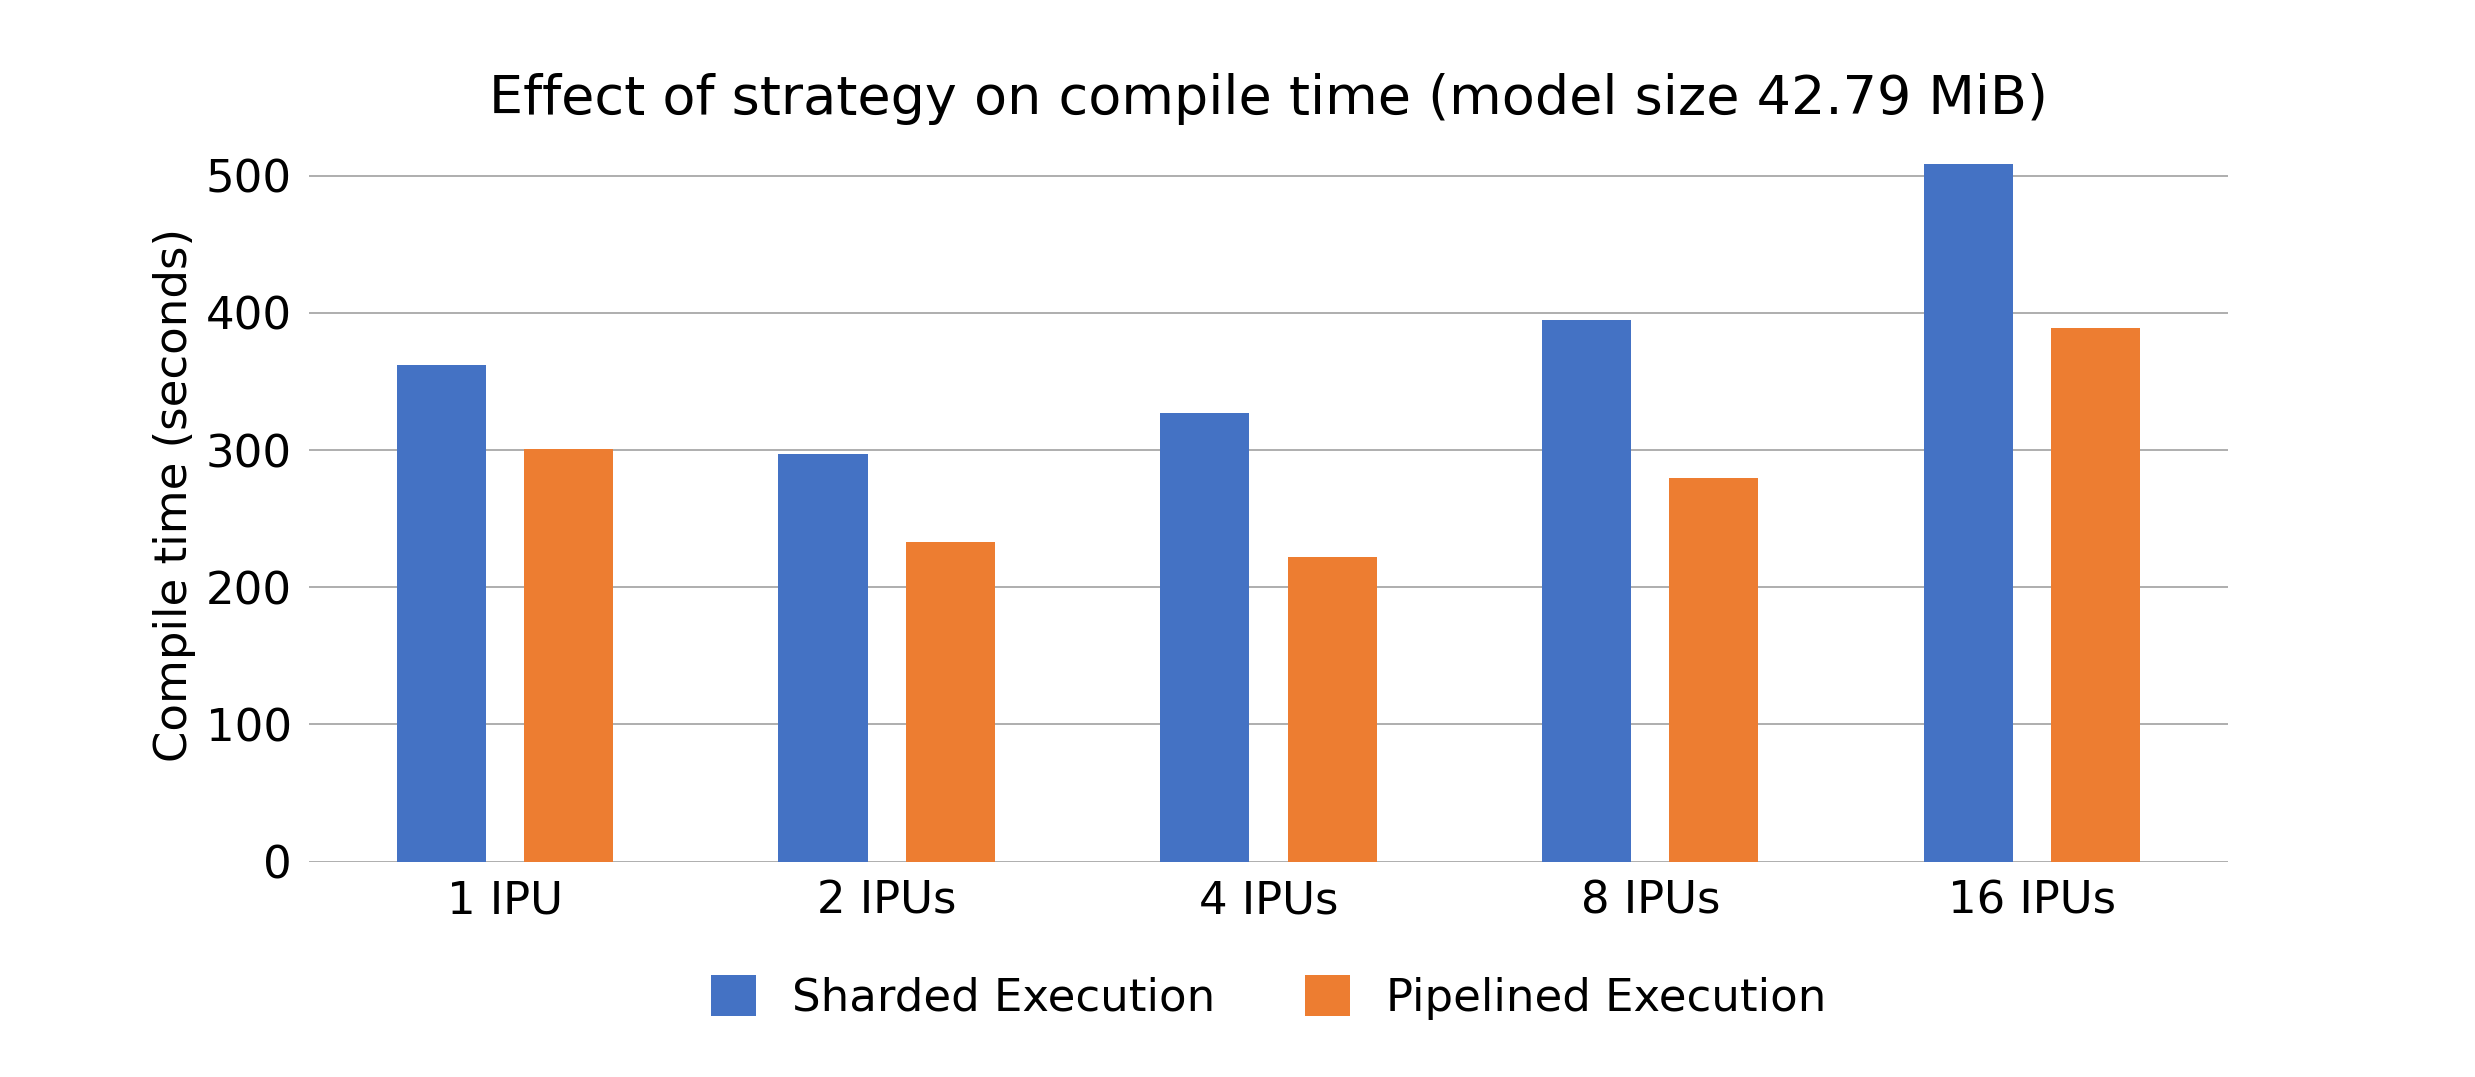
\includegraphics[width=1.0\textwidth,keepaspectratio]{6_2_1.png}
\end{frame}

\begin{frame}{Graphcore IPU-IPOD 16}
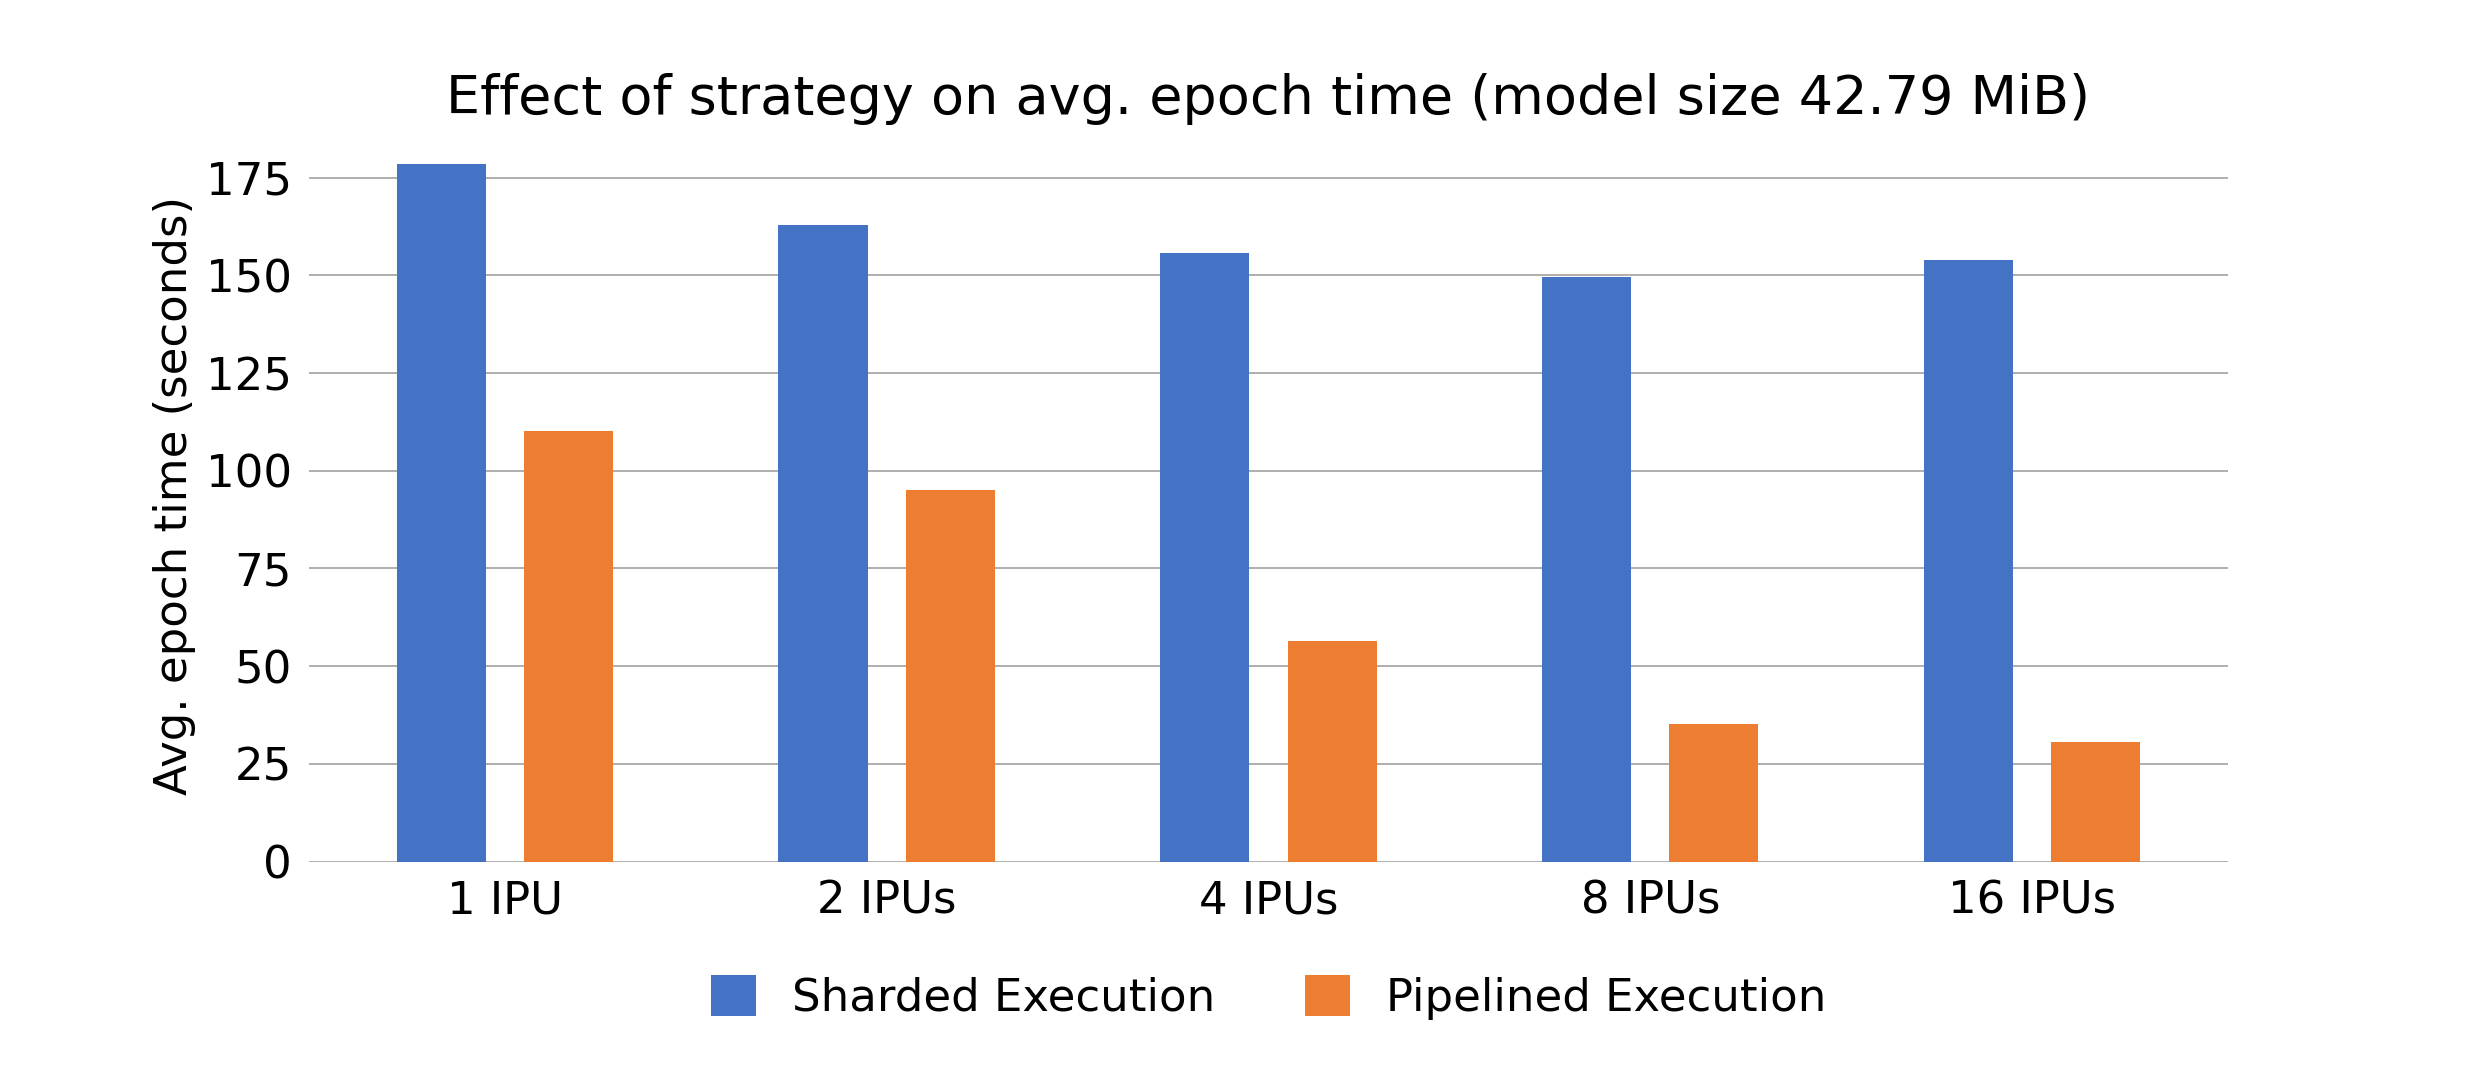
\includegraphics[width=1.0\textwidth,keepaspectratio]{6_2_2.png}
\end{frame}

\begin{frame}{Graphcore IPU-IPOD 16}
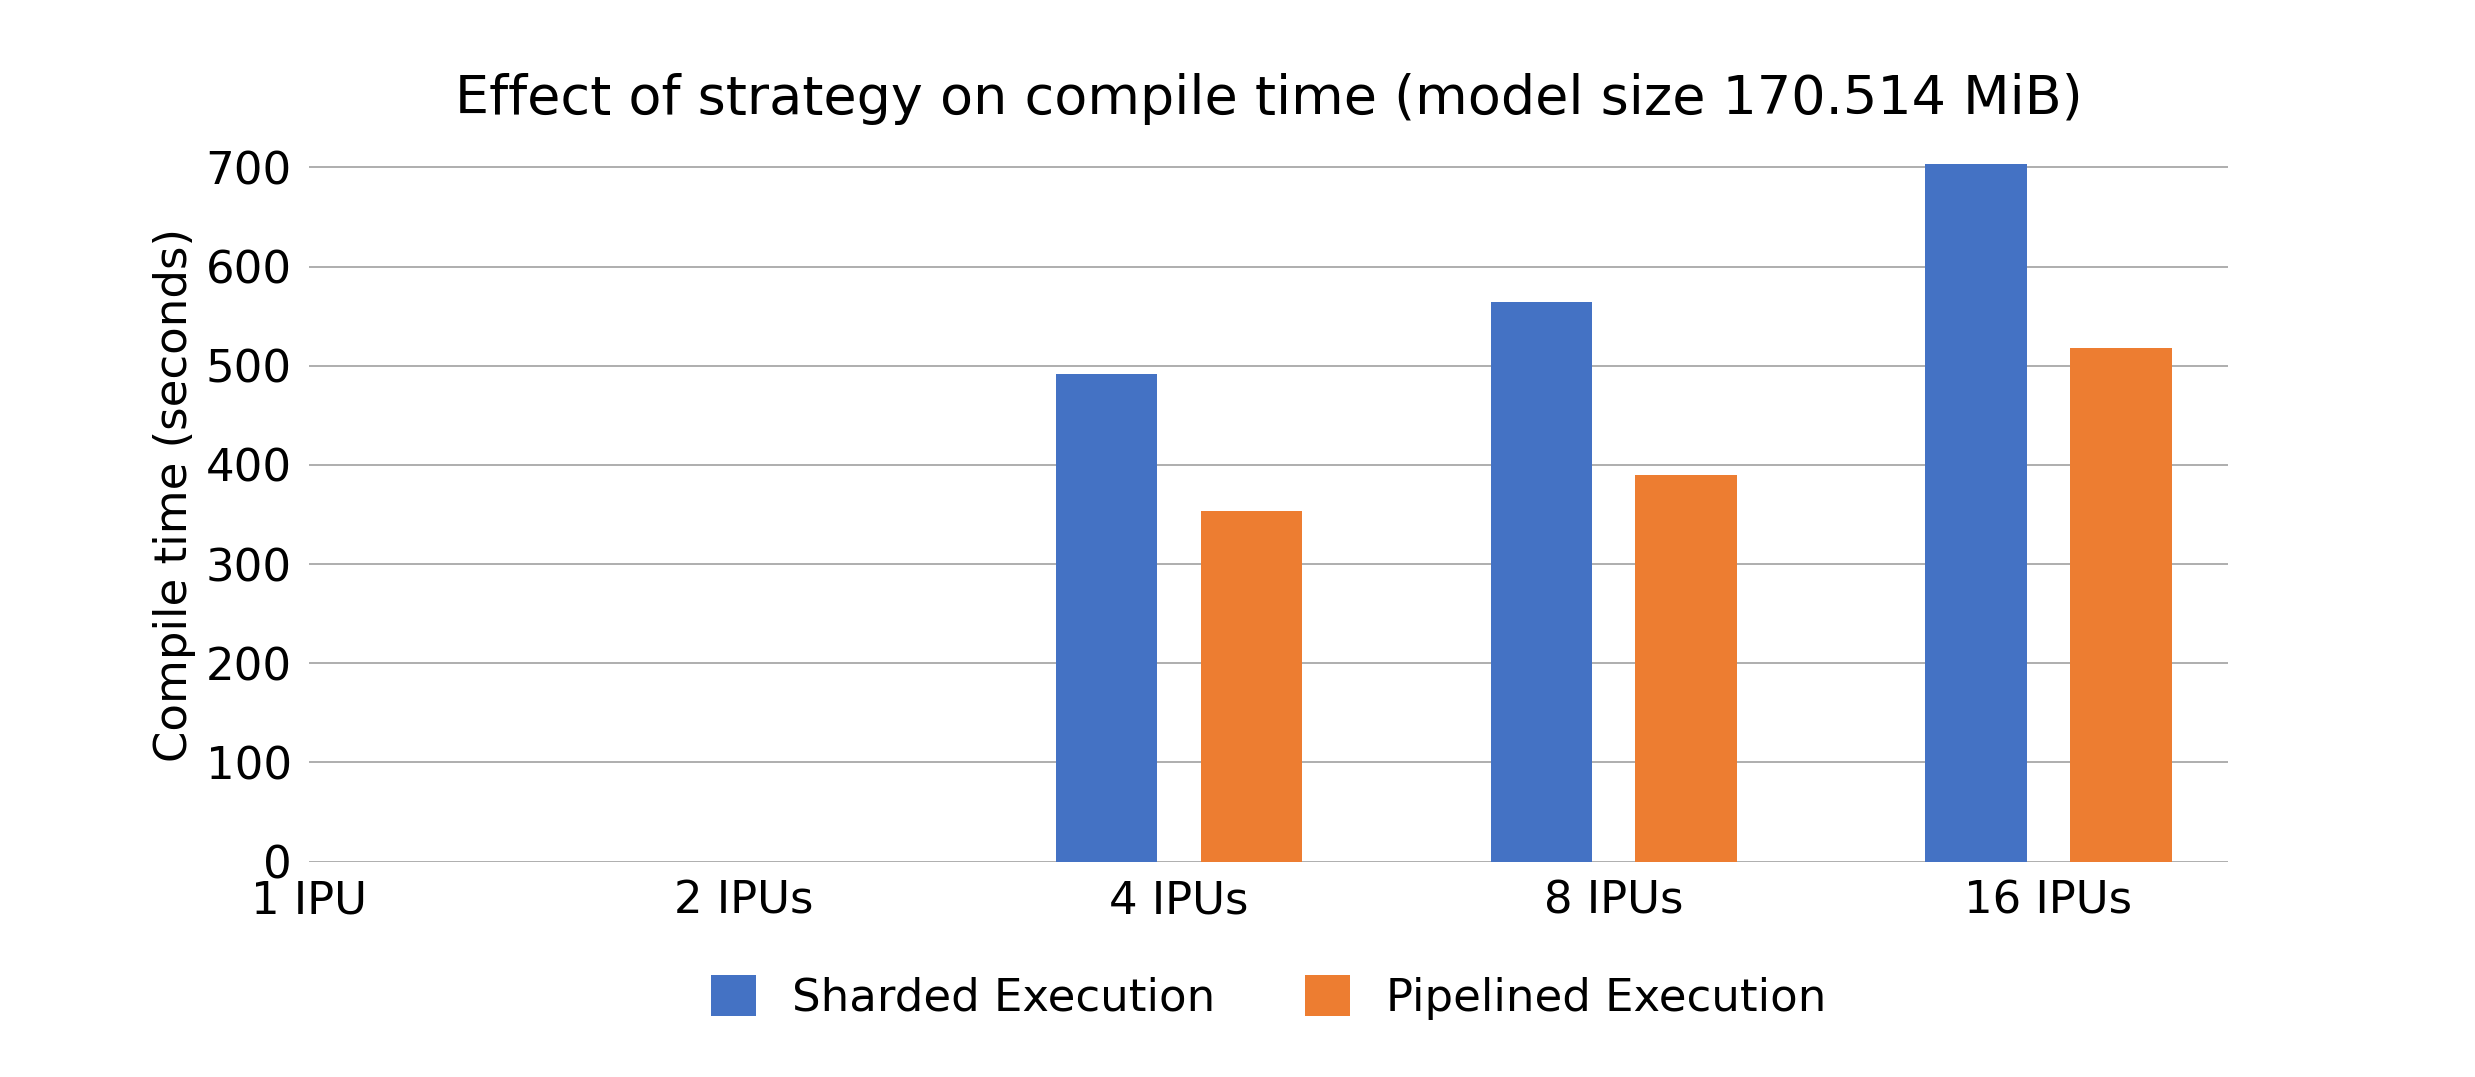
\includegraphics[width=1.0\textwidth,keepaspectratio]{6_2_3.png}
\end{frame}

\begin{frame}{Graphcore IPU-IPOD 16}
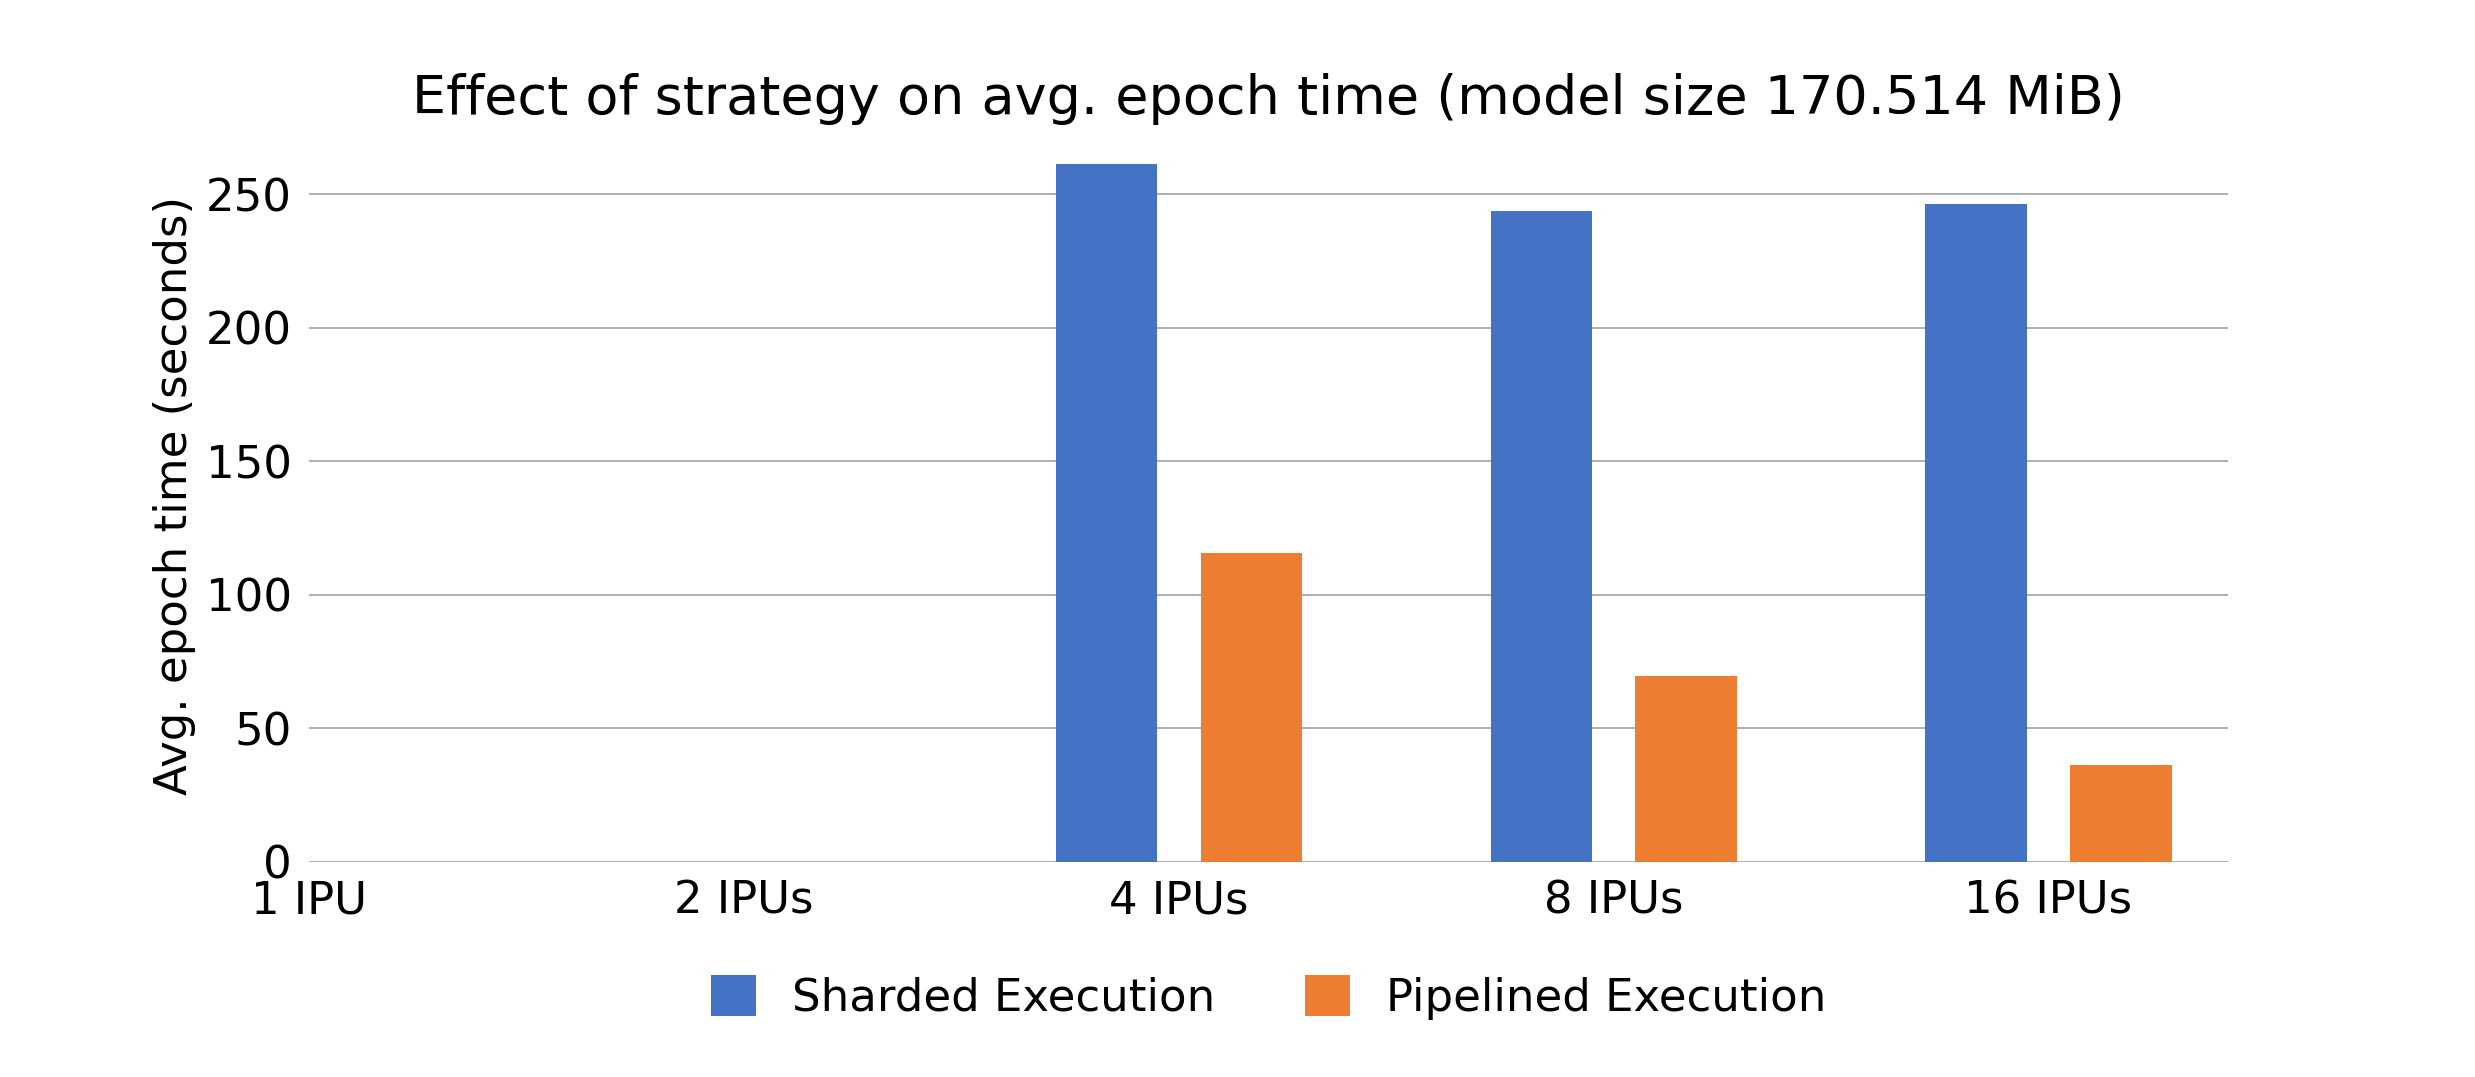
\includegraphics[width=1.0\textwidth,keepaspectratio]{6_2_4.png}
\end{frame}

\begin{frame}{Graphcore IPU-IPOD 16 - Observations}

\begin{enumerate}
  \item Compilation time increases logarithmically with IPUs for Sharded and Pipelined.
  \item Parallel Phased Execution ran on average 50 times slower than Pipelined Execution.
  \item Serial Phased Execution failed due to execution phases needing to be data-dependent.
  \item Increasing model size also causes the compilation time to increase.
  \item Epoch time decreases with the number of IPUs in use.
  \item Compilation time was nearly double the time taken to run a single training epoch.
  \item Pipelined Execution is the superior strategy.
\end{enumerate}

\end{frame}

% Section divider slide
\section{Conclusions}

\begin{frame}{Conclusions - Speed}

\begin{enumerate}
  \item BFLOAT16 peak performance is a better indicator for AI workloads than FP16 or FP32.
  \item Tensor Core on B-A100 enables mixed-precision training, better for AI workloads.
  \item C-MI100-32 and C-MI210-64 potentially more suitable for traditional HPC tasks.
  \item FSDP is faster than DeepSpeed, but DeepSpeed Stage 3 is more memory-efficient for the largest models.
\end{enumerate}

\end{frame}

\begin{frame}{Conclusions - Memory}

\begin{enumerate}
  \item DDP allows only data parallelism so model size is limited by single GPU memory.
  \item Largest model on a single B-A100-80 using DDP is GPT2-XXL; for larger models, model or pipeline parallelism is required.
  \item DeepSpeed and FSDP showed improvements in peak memory and average epoch time compared to DDP.
  \item Incrementing the GPU count consistently demonstrated diminishing average peak memory usage for DeepSpeed and FSDP.
  \item The largest model sizes that can be trained using DeepSpeed and FSDP strategies are GPT2-XXXL.
  \item A balanced consideration of both memory and time efficiency is needed especially for larger models.
\end{enumerate}

\end{frame}

\begin{frame}{Acknowledgements}

\begin{enumerate}
  \item With thanks to Edwin Brown, Sheffield and Turing.
  \item Brenden Bycroft, LLM visualisation code.
  \item This work was funded by The Alan Turing Institute under the EPSRC grant EP/N510129/1.
  \item It was partially supported by Baskerville, a national accelerated compute resource under the EPSRC Grant EP/T022221/1.
  \item It was partially supported by JADE: Joint Academic Data Science Endeavour - 2 under the EPSRC Grant EP/T022205/1, and The Exascale Computing: Algorithms and Infrastructures Benefiting UK Research (ExCALIBUR) program, which is funded under Wave 2 of the Strategic Priorities Fund (SPF).
\end{enumerate}

\end{frame}

\end{document}
